\documentclass{thomasClass}
\usepackage[utf8]{inputenc}

\usepackage[colorlinks=true, linkcolor=magenta]{hyperref}

%SETUP CODE LISTING STYLES ETC
\usepackage{listings}
\usepackage{amsmath}

\definecolor{codegreen}{RGB}{87,166,74}
\definecolor{codegray}{rgb}{0.5,0.5,0.5}
\definecolor{codepurple}{RGB}{214,157,133}
\definecolor{codeblue}{RGB}{86,156,214}
\definecolor{backcolour}{RGB}{30,30,30}
\definecolor{codenormal}{RGB}{220,220,220}

\lstdefinestyle{csharp}{
    backgroundcolor=\color{backcolour},   
    commentstyle=\color{codegreen},
    keywordstyle=\color{codeblue},
    numberstyle=\tiny\color{codegray},
    stringstyle=\color{codepurple},
    basicstyle=\ttfamily\small\color{codenormal},
    breakatwhitespace=false,         
    breaklines=true,                 
    captionpos=b,                    
    keepspaces=true,                 
    numbers=left,                    
    numbersep=5pt,
    morekeywords={abstract, as, base, bool, break, byte, case, catch, char, checked, class, const, continue, decimal, default, delegate, do, double, else, enum, event, explicit, extern, false, finally, fixed, float, for, foreach, goto, if, implicit, in, int, interface, internal, is, lock, long, namespace, new, null, object, operator, out, override, params, private, protected, public, readonly, ref,return, sbyte, sealed, short, sizeof, stackalloc, static, string, struct, switch, this, throw, true, try, typeof, uint, ulong, unchecked, unsafe, ushort, using, virtual, void, volatile, while, add, and, alias, ascending, async, await, by, descending, dynamic, equals, from, get, global, group, init, into, join, let, managed, nameof, nint, not, notnull, nuint, on, or, orderby, partial, partial, record, remove, select, set, unmanaged, unmanaged, value, var, when, where, where, with, yield},
    showspaces=false,                
    showstringspaces=false,
    showtabs=false,                  
    tabsize=2,
    rulecolor=\color{black},
    postbreak=\mbox{\textcolor{red}{$\hookrightarrow$}\space},
}
\lstdefinestyle{pseudo}{
    backgroundcolor=\color{white},   
    commentstyle=\color{codegreen},
    keywordstyle=\color{codeblue},
    numberstyle=\tiny\color{codegray},
    stringstyle=\color{codepurple},
    basicstyle=\ttfamily\small\color{black},
    breakatwhitespace=false,         
    breaklines=true,                 
    captionpos=b,                    
    keepspaces=true,                 
    numbers=left,                    
    numbersep=5pt,                  
    showspaces=false,    
    showstringspaces=false,
    showtabs=false,                  
    tabsize=2,
    rulecolor=\color{black},
    postbreak=\mbox{\textcolor{red}{$\hookrightarrow$}\space},
}
\newcommand{\inlineCode}{\lstinline[basicstyle=\small\ttfamily, breaklines=true]}

\usepackage{longtable}
\usepackage{multicol}

\usepackage{textcomp}

%MAKE PAGE HEADERS
\usepackage{fancyhdr}
\pagestyle{fancy}
\fancyhf{}
\fancyhead[LE,RO]{Thomas Boxall}
\fancyhead[RE,LO]{Virtual-Life}
\fancyfoot[RE,LO]{}
\fancyfoot[LE,RO]{\thepage}
\renewcommand{\footrulewidth}{0.4pt}

\usepackage{appendix}


%\title{A-Level Computer Science Documentation}
%\author{thomasboxall6 }
%\date{February 2022}

\makeatletter
\newcommand*{\tableofcontentssummary}{%
  \begingroup
    \value{tocdepth}=0\relax% usually show part, chapter and section only
    \@fileswfalse
    \renewcommand*{\contentsname}{Contents}%
    \tableofcontents
  \endgroup
}
\makeatother



\begin{document}

\setlength{\headheight}{13.59999pt}
\addtolength{\topmargin}{-1.59999pt}
%\maketitle
\begin{titlepage} % Suppresses headers and footers on the title page
	
	\centering % Centre everything on the title page
	
	%------------------------------------------------
	%	Top rules
	%------------------------------------------------
	
	\rule{\textwidth}{1pt} % Thick horizontal rule
	
	\vspace{2pt}\vspace{-\baselineskip} % Whitespace between rules
	
	\rule{\textwidth}{0.4pt} % Thin horizontal rule
	
	\vspace{0.1\textheight} % Whitespace between the top rules and title
	
	%------------------------------------------------
	%	Title
	%------------------------------------------------

	{\Huge \textbf{A-Level Electronics Project}}\\[0.5\baselineskip] % Title line 1
	{\huge Task 2 - Electronic System}\\[0.5\baselineskip] % Title line 2
	{\LARGE Voltmeter} % Title line 3

	
	\vspace{0.025\textheight} % Whitespace between the title and short horizontal rule
	
%	\rule{0.3\textwidth}{0.4pt} % Short horizontal rule under the title
% make a voltmeter symbol in place of short horizontal rule under the title
\begin{circuitikz}
    \centering
    \draw
    (0,0) to[rmeter, t=V] (4,0);
\end{circuitikz}
	
	\vspace{0.1\textheight} % Whitespace between the thin horizontal rule and the author name
	
	%------------------------------------------------
	%	Author
	%------------------------------------------------
	
	{\Large \textsc{Thomas Boxall}} \\% Author name
	{\large\textsc{march 2022}} % Date
	
	\vfill % Whitespace between the author name and publisher
	
	%------------------------------------------------
	%	Extra info
	%------------------------------------------------
	
	{\large\textsc{BEXHILL COLLEGE: 56635}} \\
	{\large\textsc{CANDIDATE NO: 5377}}
	
	\vspace{0.1\textheight} % Whitespace under the date text
	
	%------------------------------------------------
	%	Bottom rules
	%------------------------------------------------
	
	\rule{\textwidth}{0.4pt} % Thin horizontal rule
	
	\vspace{2pt}\vspace{-\baselineskip} % Whitespace between rules
	
	\rule{\textwidth}{1pt} % Thick horizontal rule
	
\end{titlepage}
\ \\
 \newpage
%\setcounter{tocdepth}{2}
%\tableofcontents
%\listoffigures
%\lstlistoflistings
\tableofcontentssummary

\addtolength{\topmargin}{-1.59999pt}
\setlength{\headheight}{13.59999pt}

\chapter{Analysis}
\section{Introduction}
My project will be a prototype life simulator game designed for Windows devices.\\
The project will be defined as a prototype as the scope of life simulator games is extremely broad; it will not be feasible to construct a well-rounded game in the time frame set out for this project. Due to the nature of a prototype, features may be incomplete or missing altogether. In my evaluation, I will discuss what features are incomplete or missing and ways in which they could be completed.\\
The idea for this project came from playing life simulator games and wanting to improve on them by adding a competitive aspect. This will be a single score which actions in the game will determine. The aim of the game will be to get the highest score possible. I want to design and implement this game for my project because I think it will be fun as well as a challenge; I am also interested in the balancing process which I will have to go through to make my game fair for players.


\section{Computational methods my solution will contain}
This game will be amenable to being solved using a computer program because games based off of random events are complex to develop on paper and often involve a second person to act as a 'game master', the use of a computer mitigates the need for a second person.
\subsection{Abstraction}
Real life is extremely complex and has lots of different aspects to it. This game will not have every aspect of real life programmed, so I will need to use abstraction to remove the inessential aspects of life. I will also need to use abstraction to hide some of the complex algorithms from the user, including the score calculation algorithms. \newline
An area in which I will definitely be abstracting in, is in game items. The game will not have a shop or in game wardrobe, it will just be assumed that the character has clothes. A future iteration of the game may include this.
\subsection{Decomposition}
I will need to use decomposition to break down the elements of life which I have chosen to implement into small subroutines. This will maximise efficiency as I will be able to use the same well-designed subroutine many times, minimising the number of lines of code which I have to write. By using a number of subroutines, it will mean that my program can be developed further and maintained easier after I have completed this project.
\subsection{Real time processing}
Most of this game will be fundamentally based on real-time processing. Basically everything which happens will be run in real-time as the player clicks through the game. This will need to happen quickly as it is unpleasant and off putting to use software or games where there are increased wait times for seemingly simple things. \newline
The only exception to this might be the data storage, I'm not sure exactly how I will do this, it may be run parallel to the main game code.
\subsection{Calculations}
There will be a number of time calculations are used in the game. Primarily, they will be used to run the score system, calculating the scores in real time and modifying them as and when a user changes something in the game. Calculations will also be important in deciding probabilities for certain things to happen in the game; for example, there will be an algorithm which takes the character's age as an input and returns the chance of them dying. This chance will be based off of their age and a pre-determined modifier.
\subsection{Data storage}
The data generated from each round of the game will need to be able to be saved to an external (to the game) location; for example, the C drive of the computer which the game is being run on. This will enable the player to pause their game and resume at a later time or for them to share a life with their friends over a communication platform, then their friends can install the life and play through it. The game will need to have a way for the data to be re-loaded.


\section{Stakeholders}
My target audience for this game will be casual gamers, aged between 16 and 25. Generally, I have found that this is the target audience for similar games available for different platforms. This is a broad age range, covering the upper end of the teenage market and young adulthood. I have chosen this market because I think that the content of the game will be applicable and enjoyable to those who are starting out in life (teenagers) and those who have made a start in life but could stop and pick up a different track if they wanted to (young adults). \newline
The game will be suitable to the lifestyles of teenagers as it will be designed to play in short bursts, perhaps whilst they are waiting to meet up with friends or having a break from school work. It will also be engaging for teenagers with the competitive aspect allowing them to play together to get the best score at the end of a life, sharing a screenshot from the end of the game with their peers over a communication method. There won’t be any unlockable aspects, apart from character age related content in game, so if the app has to be deleted from a device, there will be no worry about losing progress after a life is completed.\newline
The game will be suitable to young adults because it will be able to be played however they want, either making use of all the features, or playing through very simply and quickly, not making use of the features which are off the main path. This will be suitable because they might want to play the game more competitively than the teenage audience, working out the optimum way to live a life to get the best score possible, beating colleagues or friends. \newline
All users will interact with the game in the same basic way. Primarily this will be through buttons on the screens, however there will be occasional keyboard input required. The use of buttons will mean this game is suitable for those using eye tracker software or those who use touch input rather than a keyboard. The game, however, will be primarily designed for interaction using a mouse and keyboard.


\section{Research}
I had initially planned to make my game for Android devices, which is no longer possible due to software restrictions. This is why my research is aimed primarily towards mobile apps. The majority of this research will translate between Android and Windows naturally, with only very minor differences explored in the design chapter. \newline
To conduct my research for my project, I will be creating a questionnaire to send to people and researching different currently available options myself.
\subsection{Questionnaire}
I will create a Google form to send out to friends and classmates who fit into my target audience and have played games like this in the past.
\subsubsection{Questions}
I have split my questions into two categories.
\begin{enumerate}
    \item Previous experiences
    \begin{enumerate}
        \item What device(s) have you used to play Life Simulator games?
        \item What life simulator games have you played?
        \item Roughly, when did you last play this game?
        \item On average, how long do you think you played these games for?
        \item What made you stop playing these games?
        \item When you have played Life simulator games, what did you like about the game? Any specific features?
        \item When you have played Life simulator games, what did you not like about the game? Any specific features?
        \item Were there any parts of the games which you found more interesting than others? If so, what were they?
    \end{enumerate}
    \item User Interface
    \begin{enumerate}
        \item Were there any parts of the user interface which you found hard to use? What were they and what was hard to use?
        \item Were there any parts of the user interface which you found easy/intuitive to use? What were they and what was hard to use?
        \item Would you prefer a light or dark theme for the app?
    \end{enumerate}
\end{enumerate}
\subsubsection{Responses to Questionnaire}
I sent the questionnaire out to the 1st year Computer Science cohort, all of whom fit into my target audience. Listed below are the results of the questionnaire.
\begin{enumerate}
    \item 
    \begin{enumerate}
        \item 
        \begin{itemize}
            \item 33.3\% - Android phone
            \item 66.7\% - iPhone
        \end{itemize}
        \item
        \begin{itemize}
            \item BitLife (4)
            \item The Sims (2)
            \item Unnamed (1)
        \end{itemize}
        \item
        \begin{itemize}
            \item 6 months ago
            \item 2 months ago
            \item May 2021
            \item Last year.
            \item 3 years ago
            \item Maybe three years ago, 2018
        \end{itemize}
        \item 
        \begin{itemize}
            \item A fortnight
            \item A couple of months
            \item 20 mins per week
            \item 4 hours
            \item Not very much
            \item 30 mins at a time
        \end{itemize}
        \item 
        \begin{itemize}
            \item Lost interest as it started to get repetitive
            \item Glitches in software and ads
            \item Boredom/Repetitive
            \item I didn\textquotesingle t find them very interesting.
            \item The time needed for waiting
            \item Boredom
        \end{itemize}
        \item 
        \begin{itemize}
            \item Entertaining dialogue with some of the random simulations
            \item I liked being able to personalise decisions to fit my life and using it to predict my future
            \item Customisation
            \item I liked customising characters in the sims.
            \item Different types of options available
            \item How it can be a different experience each time you play, the variation
        \end{itemize}
        \item
        \begin{itemize}
            \item After a while it gets repetitive, also a lot of the the more interesting/fun features were locked behind a paywall
            \item I didn’t like when they give you options and you have to pick one of them because not all of them apply so you can’t always pick something you actually want to pick
            \item Repetitive
            \item The game itself doesn\textquotesingle t really appeal to me because I didn\textquotesingle t always have to interact with it so I spent a lot of time idle while waiting for something to happen.
            \item The camera [unsure what this is referencing]
        \end{itemize}
        \item
        \begin{itemize}
            \item The minigames for things like escaping jail etc
            \item I liked being able to see that I had to work on relationships with people (maintain friendships etc).
            \item More detailed
            \item Character customisation.
            \item The building aspect
            \item Not really
        \end{itemize}
    \end{enumerate}
    \item
    \begin{enumerate}
        \item
        \begin{itemize}
            \item Not really
            \item I don’t understand what user interface means
            \item None hard to use
            \item (Bearing in mind I haven\textquotesingle t played in ages) Some of the icons weren\textquotesingle t obvious to me so I had to click around a lot to find things.
            \item Hard - free look mode
            \item Not really
        \end{itemize}
        \item 
        \begin{itemize}
            \item Most of the UI was fairly obvious as to what it did.
            \item The Buttons were simple
            \item Icons that are easily recognisable (cog for settings, house for home/menu). The buttons had a HUD so they were easy to find.
            \item Easy - guiding character
            \item Some of the larger buttons that where perfect for the size of my phone
        \end{itemize}
        \item
        \begin{itemize}
            \item 66.7\% - Dark
            \item33.3\% - Light
        \end{itemize}   
    \end{enumerate}
\end{enumerate}

\subsubsection{Reviewing Responses To The Questionnaire}
\begin{enumerate}
    \item[1d] Time played massively varied, this could be because different people have different attention spans or they could have explored different parts of the game. The time I am attracting people to my game for is not a massive concern, however it might be an interesting to engage in a focus group with those who only played for a short amount of time to understand their answer further.
    \item[1e] It seems these responses fit into three categories: bored of playing the game; bored of waiting for things to unlock (which will allow them to progress further) and software issues, whether this be an intentional pause, paywall or glitches which made users stop playing. Ads also made the game less appealing to players, however I won't be commercialising my game so this won't be a problem.
    \item[1f] The majority of these responses suggested that the variety and randomness of the games made them appealing to play, this is something I intend on recreating in my game
    \item[1g] These responses are split into two, some not liking the repetitiveness of games like this which comes naturally when you are playing lots of lives consecutively as there are only a few routes which you can go down in a virtual life; and the second responses generally dislike a paywall feature which I wouldn’t be implementing anyway.
    \item[2a] One person commented that they found the UI hard to use, I intend to use standard icons which are well used and recognised throughout the app market to counteract this, as well as use a simple icon theme to keep my app looking tidy.
    \item[2b] Most people found the UI intuitive to use, I intend to replicate this simplicity in my own way as I think that is a very key element to having a successful app.
    \item[2c] I will be making this app with a dark theme as a default.
\end{enumerate}

\subsection{Similar Games currently available}
Before I begin to design my application, I need to look at a number of other games which are available on the app market. This will help me to understand further some of the feedback which I got from my questionnaire.
\subsubsection{BitLife}
BitLife is currently available on the \href{https://play.google.com/store/apps/details?id=com.candywriter.bitlife}{Google Play Store}.\\
The description of the app on the Google Play store outlines some features which the app has, in a handwavey way.
From playing the game, I have learnt that it allows the user to age up. When the user does this it tells them about something which has happened, for example they started at a school. Then it might prompt the user as the game goes on to pick different aspects of the life, or make decisions for the character, for example, if to kiss someone or not, if to go on a date or not. I have also learnt that many of the features of the game are only accessible after the user ages up a certain amount, this is beneficial as it keeps more to the real world as a 10 year old can’t buy a house. Furthermore, there are many other features which are accessible via a menu. There is an element of morality to the game, for example when I was playing it, I was trying to make my character go on a date with many different people even though they were married, the game prevented this every time. This game also allows you to carry on playing as your child when your character dies. Throughout the life of the character, there are events which happen - for example, a family member falls ill or dies. Another feature of the game which I like is the finance management system; part of the game is having a job which earns the character money. With that money, you are then able to purchase things - for example a house or speedboat.\\
Reading the reviews of the game suggests to me that many people are happy with the game, however some suggest that there are elements which need to be improved on for the game to be more fun, for example, someone would like there to be a one month age up option so the life of the virtual character can be explored more in depth.
The app contains in-game purchases which allow ads to be removed entirely from the game.\\
The user interface of the game is relatively messy, with adverts covering parts of the game on my phone as many buttons are placed along the bottom edge of the screen. Also, lots of the menus are very small and difficult to touch accurately 
\begin{figure}[H]
    \centering
    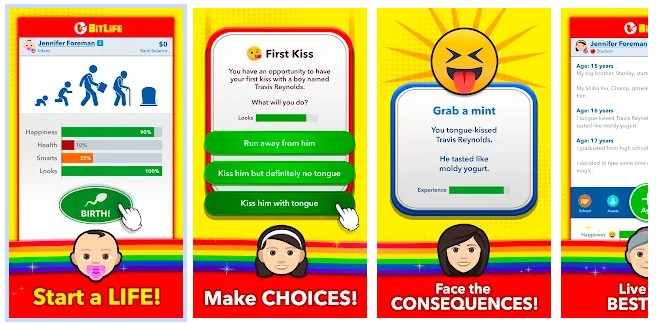
\includegraphics[width=0.9\textwidth]{images/analysis/bitLife.jpg}
    \caption{Screenshot of BitLife promotional images on the Google Play Store}
    \label{fig:bitLife}
\end{figure}

\subsubsection{Life Simulator 3}
Life Simulator 3 is currently available on the \href{https://play.google.com/store/apps/details?id=uk.playdrop.lifesimulatorpro}{Google Play store}.\\
The description of the app on the Google play store details the many elements which the game has. The main difference between this game and BitLife, is that this game allows users to create a virtual avatar whereas BitLife doesn’t.
Reading the reviews, I have learnt that there are many programmatical errors which make the game hard to play, including: when a house is sold you become “homeless” for a short while until a new house is bought, a user found that they died each time they became homeless as their health deteriorated too quickly.
Judging by the images on the Google Play store page, the user interface looks very touchscreen friendly, with big buttons and large menus where the entirety of a box is touch friendly. The images look as though the app defaults to a dark theme.
\begin{figure}[H]
    \centering
    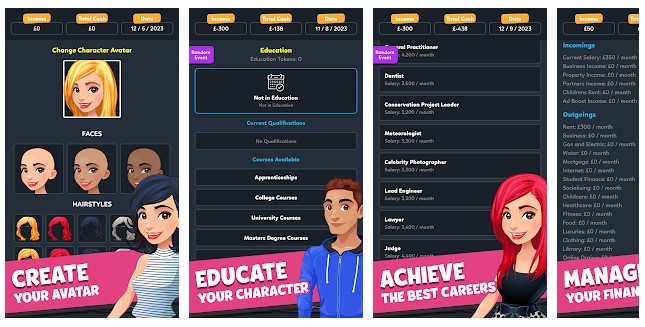
\includegraphics[width=0.9\textwidth]{images/analysis/lifeSim3.jpg}
    \caption{Screenshot of Life Simulator 3 promotional images on the Google Play Store}
    \label{fig:lifeSim3}
\end{figure}

\subsubsection{Life Simulator - Realistic Life Simulation Game}
Life Simulator - Realistic Life Simulation Game is currently available on the \href{https://play.google.com/store/apps/details?id=com.mindvacation.lifesimulator}{Google Play Store}.\\
The description of the app on the Google Play Store lists many elements which are available within the app. This app seems more modern and 'with the current times' than the others which I have looked at, containing features such as having a side hustle and a main job. It also has scenarios which set the player up to follow a specific track and achievements which can be unlocked to allow the player to do more within the app.\\
From playing this game, I have learnt that a tutorial or a clear how to play button is beneficial, which this game lacks. I spent the first 5 minutes or so trying to work out how to play the game, before stumbling across the button which makes the character older (it's a work button, not a dedicated age up button). When you do press this button, it ages you up weekly, this is shown by a tiny little dot at the top of the screen, which is not very accessible for those with a visual impairment. Also in this status bar are 3 attributes, which you have to maintain at a good level to stay alive. This is relatively challenging because to increase them, you have to spend money and when you work for money, they decrease. This is a good thing in my opinion. An improvement to this attribute display would be a percent indicator because each action has a different effect and it is hard to judge what the values in the bar are, making it hard to judge what modifier you need to apply to raise it just enough without exceeding its max value, thus wasting money. Quite a nice feature of this game, is that it doesn’t force you to follow a certain plot, even though the free version of the game forces you to pick a scenario to start the game in.\\
Reading the reviews, it seems that generally, users are happy with the game, however there are issues with the balancing of the pricing within the game.\\
The user interface of the game looks clean, with a consistent colour theme throughout the pages and greying out \& displaying a locked padlock icon for invalid buttons. It looks as though large buttons are used.
\begin{figure}[H]
    \centering
    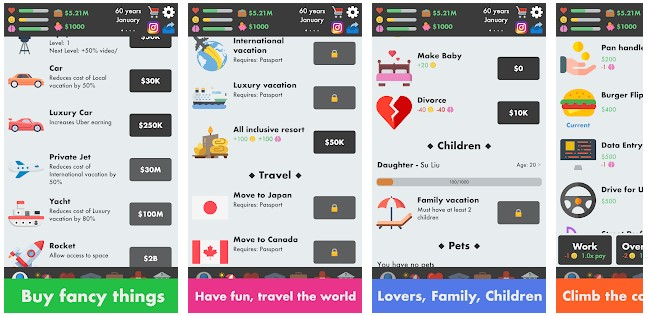
\includegraphics[width=0.9\textwidth]{images/analysis/rlsg.jpg}
    \caption{Screenshot of Life Simulator - Realistic Life Simulation Game promotional images on the Google Play Store}
    \label{fig:rlsg}
\end{figure}

\subsubsection{Reviewing Findings from Different Games}
Reviewing these similar games, it is clear that there are a few basic themes which are a constant throughout this genre of game:
\begin{itemize}
    \item Being able to make the character older
    \item Partners \& family
    \item Jobs
    \item Finance management
    \item Education
\end{itemize}
Through reviewing the games, it is clear to me there isn’t a competitive aspect to any of them. I plan on adding on to the game, through introducing a “life score”; the aim of the game is to get this score as high as possible. There will be various factors which will impact on the score.\newline
I will strive to include all of these in my final program, as well as the following which were less common amongst my research, but sound like very good ideas:
\begin{itemize}
    \item Food and diet - allowing the user to set what diet they choose for their character to dine on, this may have a financial implication if you choose for your character to eat at a hotel every day.
    \item Side Hustle - a second job which over time could progress to being the characters full time job
    \item Travelling and holidays - being able to use money earned from working to go on holiday, which improves characters attributes and opens up opportunities of finding partners with different nationalities.
\end{itemize}
There are also some elements which I really liked the look of, but will most definitely not be able to program in the time allocated for this project.

\section{Essential Features Of The Game}
\subsection{Success Criteria}
\begin{enumerate}
    \item Ageing Up
    \begin{enumerate}
        \item The game has a button which “ages up” the character
        \item As part of this process, a random event will occur (eg, family member dies, your partner wins something, you are pregnant)
        \item Some events will happen at set times (eg. finishing school)
    \end{enumerate}
    \item Relationships
    \begin{enumerate}
        \item Having a relationship with parents
        \item Having partners
        \item Marrying partners
        \item Divorcing partners
        \item Being able to pick the characters sexuality
        \item Having kids with your partner (adopted/biological)
    \end{enumerate}
    \item Crime
    \begin{enumerate}
        \item Ability to commit crime - this will be a button which will randomly generate a crime, then deduct a set amount from the lifescore.
    \end{enumerate}
    \item Employment
    \begin{enumerate}
        \item Get jobs
        \item Quit jobs
        \item The longer you stay in a job, the more \verb|jobPoints| a character will get each year. 
    \end{enumerate}
    \item Character Picker
    \begin{enumerate}
        \item At the start of each life, the user will be able to pick the character they want to play the game as. This will generate a brief backstory to the character which will crop up throughout the game (deaths of family members, key events in siblings' lives)
    \end{enumerate}
    \item Education
    \begin{enumerate}
        \item There will be a random education element to the game which will allow players to progress through school (which will have randomly generated names). Every time they complete a course or school, they get \verb|educationPoints|. 
    \end{enumerate}
    \item Saving
    \begin{enumerate}
        \item The game should be able to write the data out to a file(s) which can be loaded in during runtime to resume the game. These do not need to be readable by the user.
        \item There should be a way for the user to export the life from the game at the end of the game to a non-editable file format (eg, PDF).
    \end{enumerate}
    \item Scores
    \begin{enumerate}
        \item There should be a number of scores which the actions of the player can affect throughout the game.
    \end{enumerate}
\end{enumerate}
\subsection{Limitations of my solution}
Due to the nature of this project being a prototype which would be presented to a funding panel for assessment before further funding, there are a number of limitations of the solution.
They are outlined below.
\begin{itemize}
    \item Some aspects of the game might not be as fully fleshed out as some of the examples of similar games listed above. For example, I don’t plan on having such an intricate way of meeting partners as some of the games I played in researching; I will instead have a simple list and the player can indicate which one they wish to date;
    \item The export life function will just be to view the JSON files which the game will save data to during runtime. This will mean that definitely one element of my success criteria won't be completed;
    \item There will be a lower number of set life events, for example there will be no reference to driving lessons or other events which happen in life in a similar way;
    \item The education system will end after 6th form / college;
    \item The \verb|LifeScore| algorithm won’t be complete, however the other scores which will be the direct source of information for the \verb|LifeScore| will be complete;
    \item The marriage section of the game will not be implemented.
\end{itemize}

\section{Hardware Requirements}
As the application will be developed using Visual Studio 2019, the minimum software requirements will be the same as Visual Studios requirements:
\begin{itemize}
    \item 1.8 GHz or faster processor. Quad-core or better recommended;
    \item 2 GB of RAM; 8 GB of RAM recommended (2.5 GB minimum if running on a virtual machine);
    \item Hard disk space: Minimum of 800MB up to 210 GB of available space, depending on features installed; typical installations require 20-50 GB of free space;
    \item Hard disk speed: to improve performance, install Windows and Visual Studio on a solid state drive (SSD);
    \item Video card that supports a minimum display resolution of 720p (1280 by 720); Visual Studio will work best at a resolution of WXGA (1366 by 768) or higher.
\end{itemize}


\chapter{Design}

\section{Specification}
\begin{enumerate}
    \item The traffic light control system should be easy to use.
    \item The traffic light control system should be as efficient as possible, reducing heat dissipated to the environment.
    \item The traffic light control system should recieve an input from a pedestrian and take 40 seconds ($\pm$20s) to allow them to cross.
    \item The traffic light control system should not favour any particular road user over an other as well as giving equal chances to all direction of traffic.
    \item The traffic light system should ensure that when a direction of traffic is not able to go, its red stop LED is illuminated.
    \item The traffic light control system should take a 0V and +5V (within $\pm$0.5V) input.
    \item The traffic light control system should alert 'pedestrians' in at least two different ways that it is their turn to cross.
    \item The traffic light control system should be developed in a way such that, the code is clear to read and understand, to ensure future developments can be carried out easily.
\end{enumerate}

\section{Junction design}
Now I have my specification, I am able to design the junction which I will design the traffic light control system for. I will be using a junction in my home town (Eastbourne) as inspiration.
\subsection{Real Life Junction}
\begin{figure}[H]
    \centering
    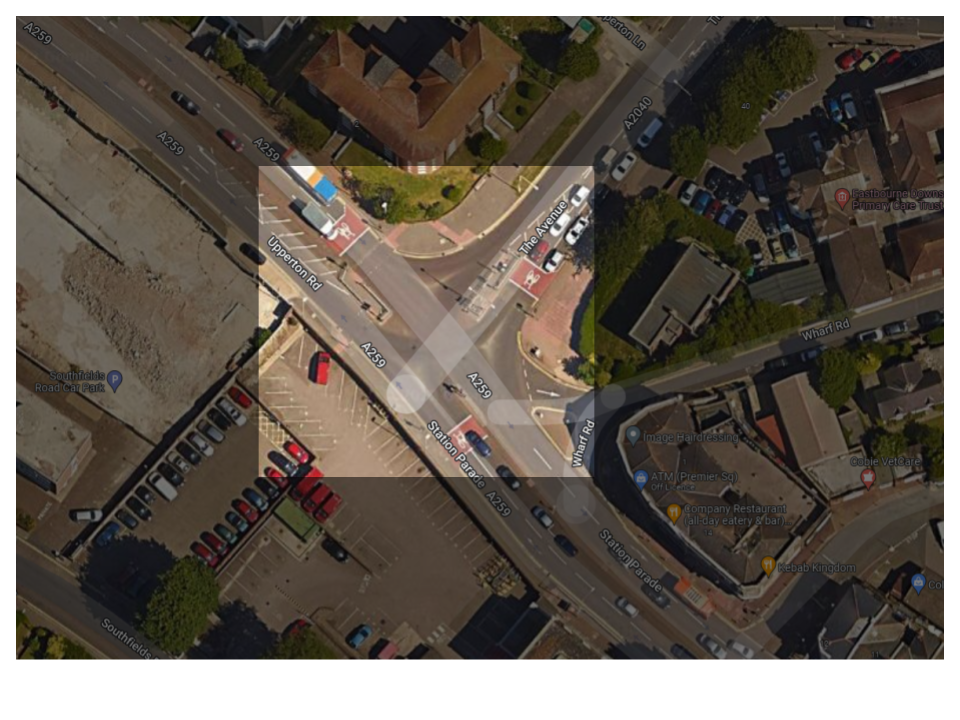
\includegraphics[width=0.9\textwidth]{images/IRL diagram.png}
    \caption{Image of the inspiration junction}
    \label{fig:IRLJunction}
\end{figure}
\noindent \textit{Data from Google Maps (2022). Available from:\\ https://www.google.com/maps/@50.7701274,0.2786944,118m/data=!3m1!1e3 [Accessed 13 03 2022]}\newline

\noindent This is a three-way traffic light controlled junction with pedestrian crossing for two of the three ways. 

\subsection{Abstracted Junction}
\begin{figure}[H]
    \centering
    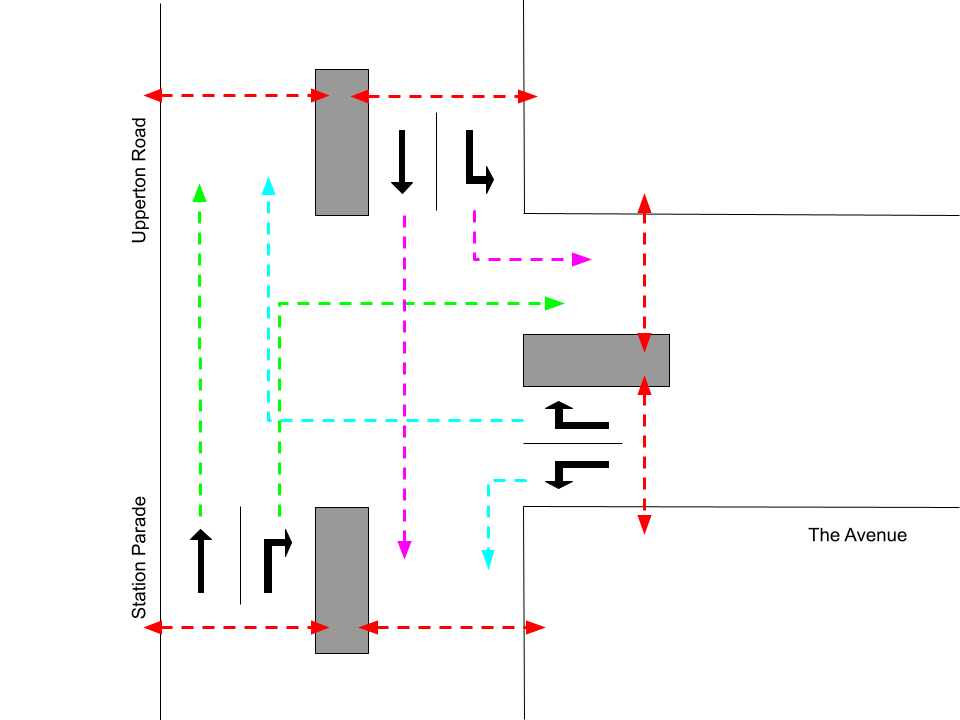
\includegraphics[width=0.8\textwidth]{images/Abstracted diagram.png}
    \caption{Diagram of the junction used in this project}
    \label{fig:abstractedDiagram}
\end{figure}
\noindent The diagram above shows an abstracted version of the junction shows in figure \ref{fig:IRLJunction}. This abstracted version has four colours dashed lines drawn on it. These show the routes which can be taken by either the pedestrians or cars. The red route indicates a pedestrian crossing. The blue, pink and green lines indicate routes which can be taken by vehicles. The grey boxes indicate pedestrian islands. Additional pedestrian crossing routes have been included in my abstracted diagram. This is because in the real junction, the areas which do not have pedestrian crossings are extremely dangerous as cars travel at high speeds.

\section{Traffic Light Sequence}
After working out the type of junction I will design an traffic light control system for, I am now able to work out the sequence which the traffic lights will cycle through. At this point, I have also decided that the traffic light sequence will be contained within a subroutine; hence the references about 'Main Program' in the diagram below.
\begin{figure}[H]
    \centering
    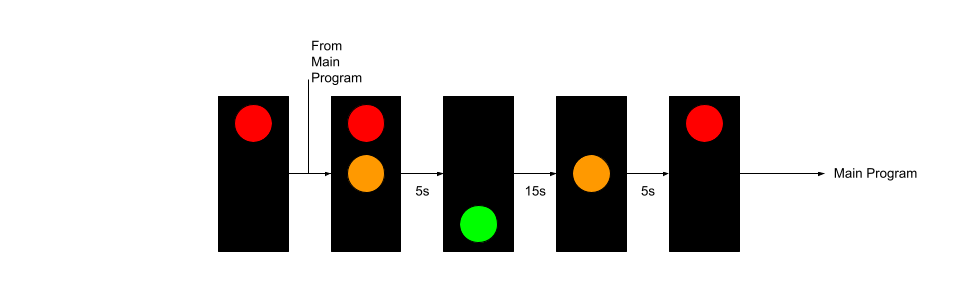
\includegraphics[width=0.9\textwidth]{images/Traffic light sequence.png}
    \caption{Sequence of lights in the traffic lights}
    \label{fig:trafficLightSequence}
\end{figure}

\section{Inputs and Outputs}
The PIC16F88 microcontroller has 16 input output bits, divided into two 'ports' of 8 (PORTA and PORTB).
In my system, all inputs and outputs will be active high (logic 1).
\begin{figure}[H]
    \begin{minipage} {0.45\textwidth}
        \subsection{PORTA}
        \begin{itemize}
            \item[0] Output, red LED
            \item[1] Output, amber LED
            \item[2] Output, green LED
            \item[3] Output, red LED
            \item[4] Output, amber LED
            \item[5] 
            \item[6] Output, red LED
            \item[7] Output, amber LED
        \end{itemize}
    \end{minipage}\hfill
    \begin{minipage} {0.45\textwidth}
        \subsection{PORTB}
        \begin{itemize}
            \item[0] Output, green LED
            \item[1] Input, button
            \item[2] Output, white LED
            \item[3] Output, red LED
            \item[4] Output, green LED
            \item[5] Output, buzzer
            \item[6] 
            \item[7] Output, green LED
        \end{itemize}
    \end{minipage}
\end{figure}


\section{Component of the control system}
The control system will be based off of a PIC16F88 microcontroller, this will be the heart of the system. Alongside the microcontroller, I will also need some LEDs (in red, amber and green), a buzzer and a button.
\subsection{Components list}
\begin{itemize}
    \item 4 red LEDs
    \item 4 green LEDs
    \item 3 amber LEDs
    \item 1 white LED
    \item 2 eight 220K$\Omega$ resistor packs
    \item 3 220k$\Omega$ resistors
    \item 1 1K$\Omega$ resistor
    \item 1 Push-To-Make button
    \item 1 PIC16F88 Microcontroller
\end{itemize}
In reality, my circuit will only need 12 220K$\Omega$ resistors. However, for convenience, and minimising the number of components on the breadboards, it is easier to use 2 resistor packs and a number of loose resistors.



\chapter{Testing During Development}
During the development of my project, I will need to evaluate each section I program against my success criteria to ensure it works. I will also need to ensure that there are no bugs or errors in the code.
\section{Types of Testing Used}
To test my code as I go along, I will be using the following types of testing;
\begin{itemize}
    \item White Box testing
    \item Integration testing
\end{itemize}
Each type of testing has a different strength. White box testing will allow me to test each programmatic element as I go along as I will know how it should be Integration testing will allow me to test how the different subroutines of the program interface with each other and confirm that data is being passed between them correctly.

\section{Important elements to test during development}
Listed below are the elements of my project which will need to be individually tested before they can be combined into the main game.
\begin{itemize}
    \item Buttons on the forms\\
    The buttons on the forms will need to work correctly.
    \item Generation of classes\\
    The classes will need to be constructed correctly.
    \item Files\\
    The game will need to be able to save data out to files then read it back in.
    \item Events\\
    The events in the game will need to be generated and displayed correctly.
    \item Generation of people\\
    Both the family members and potential partners need to be generated randomly. These can be tested separately by using message boxes to display information from each person.
    \item Death\\
    The death algorithms will need to randomly select a character to die and them kill them.
    \item Scores \\
    The scores will need to be calculated and displayed correctly.
    \item Education\\
    The education system will need to work as designed my success criteria. This will be programmed in a modular way, so each subroutine can be tested before testing the subsystem as a whole.
    \item Crimes\\
    The crimes element will need to work independent of any other system in the game before it is combined.
    \item Jobs\\
    This subsystem, can be tested fully on its own before being integrated with the rest of the game.
    \item Partners\\
    The partners element to the game can't be tested fully independently because it will make use of some of the same functions which are used in the generate family members systems. This, however, shouldn't be a problem.
\end{itemize}

\section{Post Development Testing}
After I have completed implementation of the project, I will need to test the complete program to ensure that all the different systems work together correctly. I will be using the test plan detailed in chapter \ref{chap:testPostDev}. 
\UseRawInputEncoding
\chapter{Implementation}
I will be implementing my project using Microsoft Visual Studio 2019 within a Windows Executable application template using the .NET Core framework version 3.1. \newline
The first form I will design is the main menu as this is what the players will see first when they open the game.

\section{Designing the Main Menu}
I began by setting up the form background colour then added the panel controls then I added the rest of the controls to the screen. I made sure to give all the controls which would have events associated to them in the code a meaningful name, to ensure I could address them without confusion of which control was which. For example, the button which loads a new game is called \verb|btnNewGame| (screenshots of the forms annotated with the control names are available in Appendix \ref{app:ScreenshotsOfForms}).\\
I also made sure that the controls on the forms responded dynamically to the size of the window to make sure that as the window was resized, the controls would move to the centre.
The final main menu form (design) is shown below:
\begin{figure}[H]
    \centering
    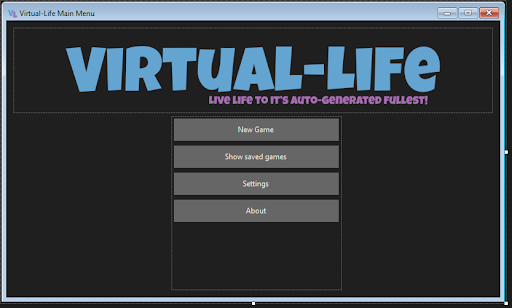
\includegraphics[width=0.8\textwidth]{images/implementation/mainMenu.png}
    \caption{Main menu form design}
    \label{fig:implementation-mainMenu}
\end{figure}

\section{Declaring Classes and Passing Objects Between Forms}
Now that I have a basic user interface (UI) designed, I am able to begin programming the game which will run behind it. I will start with moving an object between forms. This is fundamental to my game as I will be constructing an object in one form then moving it to another form where it will be processed. It is important that the object along with all its attributes is moved in its entirety. This means that as the game progresses from the new game screen to the main game play form, the objects already generated are accessible. \newline
To work out how to do this was quite a complicated process as there were lots of different out of date tutorials on the internet, it taught me the importance of testing small elements of the code in a test project before moving them into the main program.
\begin{lstlisting}[language=c, style=csharp, caption=Displaying a new form and passing an object to it]
frmMainGameScreen fMainGameScreen = new frmMainGameScreen(mainCharacter); //create new frmMainGameScreen with parameter mainCharacter
fMainGameScreen.Show(); //show new main game screen.
\end{lstlisting}
\noindent The code above creates the new instance for \verb|frmMainGameScreen| and passes into the constructor the \verb|mainCharacter| object. The \verb|mainCharacter| object is passed from form to form throughout the program.\\
The code below takes the object (being passed into the new form) as a parameter of the constructor of the form.
\begin{lstlisting}[language=c, style=csharp, caption=New form constructor code containing processing for object being passed in as a parameter]
public frmMainGameScreen(Person mainCharacterTransfer)
{
    InitializeComponent();            
    mainCharacter = mainCharacterTransfer; //Set the contents of mainCharacter to mainCharacterTransfer which has come from previous form
}
\end{lstlisting}

\section{Creating the Person classes}
Using my class diagrams, I then setup the rest of the classes and setup the inheritance for the classes relating to people. For now, I have only inputted the attributes for the classes, methods will be setup later as I need them.
\begin{lstlisting}[language=c, style=csharp, caption=GenericFamilyMember class creation]
 public class GenericFamilyMember : Person
{
    private string relationshipToMain;

    //get and set
    public string RelationshipToMain { get; set; }
}
\end{lstlisting}
\begin{lstlisting}[language=c, style=csharp, caption=MainCharacter class creation]
public class MainCharacter : DetailedCharacter
{
    //attributes

    private int expenses;
    private int bankBalance;
    private int jobBand;
    private string jobTitle;
    private int jobSalary;
    private int jobCurrentDuration;
    private int salary;

    //get and set
    public int Expenses { get; set; }
    public int BankBalance { get; set; }
    public int JobBand { get; set; }
    public string JobTitle { get; set; }
    public int JobSalary { get; set; }
    public int JobCurrentDuration { get; set; }
}
\end{lstlisting}
\begin{lstlisting}[language=c, style=csharp, caption=Partner class creation]
public class Partner : DetailedCharacter
{
    Random rnd = new Random();
    private string whereMet;
    private DateTime whenMet;

    //get and set
    public string WhereMet { get; set; }
    public DateTime WhenMet { get; set; }
}
\end{lstlisting}
\begin{lstlisting}[language=c, style=csharp, caption=Person class creation]
public class Person
    {
        //Set all private attributes for the class
        private string firstName;
        private string lastName;
        private string gender;
        private string sexuality;
        private int age;
        private bool livingStatus;
        private DateTime dateOfBirth;
        private DateTime dateOfDeath;
        private string reasonForDeath;
        private bool inRelationship;
        //get and set methods (nb. use uppercase first character for accessable get/set)
        public string FirstName { get; set; }
        public string LastName { get; set; }
        public string Gender { get; set; }
        public string Sexuality { get; set; }
        public int Age { get; set; }
        public bool LivingStatus { get; set; }
        public DateTime DateOfBirth { get; set; }
        public DateTime DateOfDeath { get; set; }
        public string ReasonForDeath { get; set; }
        public bool InRelationship { get; set; }
    }
\end{lstlisting}
\section{Working More on The Forms}
Now I had the basics worked out (how to pass data from one form to another and accessing objects in C\#), I designed the new game and show saved games form. Both of these forms are fundamentally the same, with each having text boxes for the attributes of the main character. However, on the show saved games form, the text boxes are read only and they get populated once the user has opened the file.
\begin{figure}[H]
    \centering
    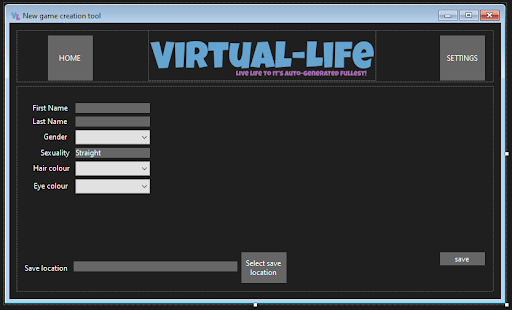
\includegraphics[width=0.8\textwidth]{images/implementation/newGameForm.png}
    \caption{Create new game form}
    \label{fig:implementation-newGameForm}
\end{figure}
\noindent The figure below shows the show saved games form. It contains text box controls which will be used to show the main characters information to the player, this will allow them to confirm that they have selected the correct save before the computer loads the data then then the game progresses to the next form.
\begin{figure}[H]
    \centering
    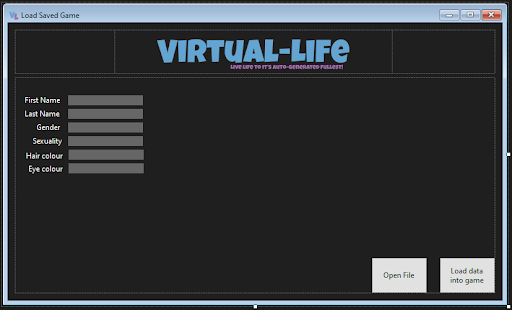
\includegraphics[width=0.8\textwidth]{images/implementation/showSavedGamesForm.png}
    \caption{Show saved games form}
    \label{fig:implementation-showSavedGamesForm}
\end{figure}

\section{File Handling}
One of the key elements of my success criteria was the ability to save a game to a file and read it back in when the app was opened again. \\
As I had worked with JSON files in previous projects before, I decided to use them for this project as I understood how to use them effectively. I did some research into saving to a JSON file and found a package called Newtonsoft. This package can serialize and deserialize the JSON file. The documentation for the package is bad at explaining why things work, so I spent quite a lot of time working out how to manually write the contents of each object out to an individual JSON file before I realised that part of the package might be able to do that for me. \newline
This is on my to-do list as a lower priority task as I feel like I'm focusing on the small details too much and not working on the actual game. I have also got a single object read back in by the program, however this is the only object in the file so I'm not sure if the same code will work when I introduce different objects to the file. At this moment in time, this isn\textquotesingle t meeting my success criteria.

\section{Loading Bar}
This wasn't in my design, however I believe it adds some value to the game, especially when handling files as wait times could be increased on slower systems.\\
It is a small form which appears with a marquee scrolling progress bar which says "Loading" on it, to tell the user that the game is doing something when the program is doing something; for example, when it is saving to a file.\\
The progress bar begins to move automatically, this is setup in the control properties within Visual Studio.
\begin{figure}[H]
    \centering
    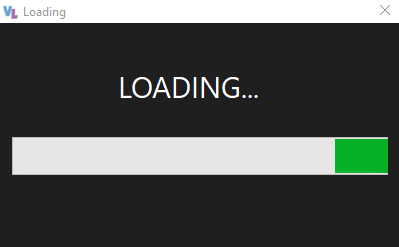
\includegraphics[width=0.4\textwidth]{images/implementation/loadingBarForm.png}
    \caption{Loading bar form}
    \label{fig:implementation-loadingBarForm}
\end{figure}

\begin{lstlisting}[language=c, style=csharp, caption=Code for the loadingbBar form]
public partial class frmLoadingBar : Form
{
    public frmLoadingBar()
    {
        InitializeComponent();
    }
}
\end{lstlisting}

\section{Building Main Game Screen form}
I began to build the form for the main game screen, by adding the TabControl which will allow me to have different tabs of information on one form, reducing the number of different forms which have to be loaded into memory at the same time; this also produces all-on-one-screen design which many of the games I played in research had.\\
After the TabControl, I added more panel controls to separate the different boxes of the information, to make resizing the form dynamically easier.
\begin{figure}[H]
    \centering
    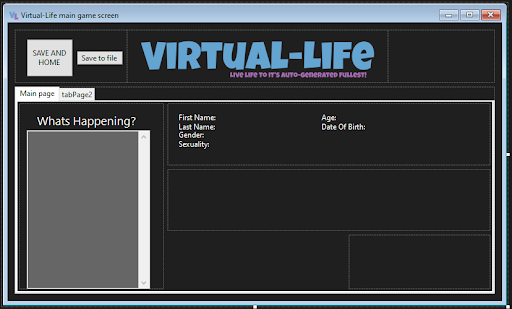
\includegraphics[width=0.8\textwidth]{images/implementation/buildingMainGameScreen.png}
    \caption{Work in progress of main game screen form}
    \label{fig:implementation-buildingMainGameScreen}
\end{figure}

\section{Array of Event Objects}
To store the various events I will have throughout the game, I will be creating an object for each one and to make programming and future maintenance easier, I will be storing them in an array.\\
I first wrote the code which made it work on one form. This worked the first time as I was following a tutorial and looking at errors which Visual Studio was giving me; correcting them as I programmed more. Then I setup the constructor for the next form in the game (main game screen) to receive the array of events object.
\begin{lstlisting}[language=c, style=csharp, caption=First attempt at declaring an array of objects]
Event[] eventArray = InitializeArray<Event>(numberOfEvents);
\end{lstlisting}
This resulted in the following error:\\
\verb|A field initializer cannot reference the non-static field, method, or property|\\ \verb|'frmNewGame.numberOfEvents'|\\
To fix this, I tried removing the variable numberOfEvents and changing it to a static integer like so:
\begin{lstlisting}[language=c, style=csharp, caption=Second attempt at declaring an array of objects]
Event[] eventArray = InitializeArray<Event>(10);
\end{lstlisting}
This still gave me the following error:\\
\verb|A field initializer cannot reference the non-static field, method, or property|\\ \verb|'frmNewGame.InitializeArray<Event>(int)'|\\
To try to fix this, I ignored the InitializeArray function and just declared a new array of objects:\\
\begin{lstlisting}[language=c, style=csharp, caption=Third attempt at declaring an array of objects]
public Event[] eventArray = new Event[10];
\end{lstlisting}
However, this gave me a null error saying the objects aren't defined.\\
I reverted back to the previous way and did some research - this pointed me at a Microsoft Docs page detailing Compiler Error CS0236.\\
From previous knowledge, I realised that compiler errors aren't something which are simple to understand, so I tried another option.\\
This gave me the following error:
\inlineCode{System.NullReferenceException:' Object reference not set to an instance of an object.' }\\
To resolve this error, I did more research and settled on the following solution.\\
This first block of code comes from when the new game screen form is loaded.
\begin{lstlisting}[language=c, style=csharp, caption=Final solution for declaring an array of objects part 1]
//Create array of event object called eventArray
public int numberOfEvents = 1000;
public Event[] eventArray = new Event[1000];
public int nextEvent = 0;
\end{lstlisting}
This next block of code is run when the save button is pressed
\begin{lstlisting}[language=c, style=csharp, caption=Final solution for declaring an array of objects part 2]
//create event objects needed for game
for (int i = 0; i < controlClass.NumberOfEvents; i++)
{
    eventArray[i] = new Event();
}
\end{lstlisting}
This works by setting up the integer variable \verb|numberOfEvents| then the array of type \verb|Event| containing 1000 \verb|Event| objects and then the integer variable \verb|nextEvent| which would be used to find the next available slot in the array meaning I could very quickly input the next item in the array without having to locate it every time I needed to enter something into it. The \verb|numberOfEvents| variable could be set dynamically using an inbuilt C\# method for array handling - my intention is to change this over. This change would mean that I would only need to change the length of the array once in the program and the change would be reflected all throughout the code.
After I had added the code which is needed to populate the array:
\begin{lstlisting}[language=c, style=csharp, caption=Code needed to create the first event in the array]
eventArray[controlClass.NextEvent].Category = "Life Event";
eventArray[controlClass.NextEvent].DateHappened = DateTime.Today;
eventArray[controlClass.NextEvent].Description = "You were born to parents xxx;
controlClass.NextEvent++;
\end{lstlisting}
I tested it and I got the outcome which I wanted to see - the text box on the main game screen showing the event.
\begin{figure}[H]
    \centering
    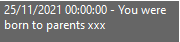
\includegraphics[width=0.4\textwidth]{images/implementation/eventArrayDemo.png}
    \caption{Evidence that the array of Event objects are being constructed correctly}
    \label{fig:implementation-eventArrayDemo}
\end{figure}

\section{File Handling - Attempt 2}
When I worked on loading the saved files into the game, I realised that the JSON package handler I was using had a serialisation and deserialization function built in which is much more elegant and resource efficient than the method which I was using. I looked into the different methods which came with \verb|Newtonsoft.Json| and found the \verb|JsonConvert.SerializeObject(objectName)| and tested writing out to a file using that. This worked first time with the following code.
\begin{lstlisting}[language=c, style=csharp, caption=Code used to write out to JSON files]
File.WriteAllText(filepath, JsonConvert.SerializeObject(mainCharacter));
\end{lstlisting}
However, I also had to include \verb|Newtonsoft.Json| separately to \verb|Newtonsoft.Json.Linq| at the top of the project. I then began to look at how to write out the other objects to the file.
It was extremely difficult to get the writing out and reading in working. I spent a lot of time following tutorials which ended in an error or not the result I was expecting. I decided that to make this work, I would need to go back to basics and work out exactly what I needed, not what I wanted. This re-designing allowed me to realise that there was no need for all the objects to be written out to the same file, they could be in fact written out to separate files within one folder. This epiphany resulted in me solving how to get the objects written out to separate files, and read them in again. To write them out, I did it in much the same way as before however, in my \verb|File.WriteAllText| statement, I also had to include the file name. The code below shows how a single object is written out to a JSON file. This is repeated multiple times in the code with the filepath and object name substituted.
\begin{lstlisting}[language=c, style=csharp, caption=Code used to write out to JSON files]
File.WriteAllText(controlClass.Filepath + "\\mainCharacter.json", JsonConvert.SerializeObject(mainCharacter));
\end{lstlisting}
This was much the same for when a file is being opened.
\begin{lstlisting}[language=c, style=csharp, caption=Code used to open a JSON file and read the contents of it into an object]
MainCharacter mainCharacter = JsonConvert.DeserializeObject<MainCharacter>(File.ReadAllText(loadFilepath + "\\mainCharacter.json"));
\end{lstlisting}
To select the folder which I was going to be using, I used a FolderBrowserDialog control which comes as standard with the Windows Form Library.

\section{Control Class}
Whilst designing the file management system, I realised that there were lots of data items which would need to be stored alongside the game for the game to work. Up until now, I had been storing them as variables but hadn't thought about how I would need to save them. I decided to save them as an object, this way I can easily save to a file in the same way I am doing for the other objects.
This control class also means I am able to pass data between forms much simpler, as I can simply pass the entirety of the \verb|controlClass| to the new form rather than the individual attributes separately.
\begin{lstlisting}[language=c, style=csharp, caption=Declaration of Control Class]
public class ControlClass
{
    //private attributes
    private DateTime inGameDate;
    private int numberOfEvents;
    private int nextEvent;
    private string filepath;
    private int numberOfFamily;
    private int nextFamily;
    private string nameOfCurrentSchool;
    private int currentSchoolYear;
    private int eduScorePlus;
    private int happinessScorePlus;


    //get and sets
    //GENERIC GAME STUFF----
    public DateTime InGameDate { get; set; }
    public string Filepath { get; set; }
    //EVENTS-------
    public int NumberOfEvents { get; set; }
    public int NextEvent { get; set; }
    //FAMILY--------
    public int NumberOfFamily { get; set; }
    public int NextFamily { get; set; }
    //EDUCATION------
    public string NameOfCurrentSchool { get; set; }
    public int CurrentSchoolYear { get; set; }
    public int EduScorePlus { get; set; }

    //HAPPINESS SCORE-----
    public int HappinessScorePlus { get; set; }

}
\end{lstlisting}

\section{Random Generation of Family Members}
I decided that I would be using the constructor of the \verb|GenericFamilyMember| class to populate the attributes of each object. To differentiate between each family member, I will be passing into the constructor the number in the \verb|familyArray|, allowing me to use a switch statement to differentiate between family members.\\
To start with, I am using 2 attributes of index 0, which is the father of the main character. This will allow me to test the random generation aspect (in the \verb|FirstName| attribute) and the fixed value aspect (in the \verb|RelationshipToMain| attribute).\\
I wrote the following code.

\begin{lstlisting}[language=c, style=csharp, caption=Initial test of generating a Random Character]
public GenericFamilyMember(int charNumber)
{
    //construct here
    //go through a switch statement to set the character based on what their relationship to the main is.
    switch(charNumber)
    {
        case 0:
            //Dad to main character
            FirstName = genMFN();
            RelationshipToMain = "Father";
            break;
        default:
            FirstName = null;
            break;
    }
}

//Generate a Male first name
public static string genMFN()
{
    //generate male first name
    string[] name = { "Liam", "Noah", "Oliver", "Elijah", "William", "James", "Benjamin", "Ben", "Lucas", "Henry", "Alex", "Ethan", "Daniel", "Sebstian", "Jack", "Matt", "John", "Joe", "David", "Josh", "Julien", "Leo", "Isaac", "Thomas", "Max", "Andy", "Phill", "Harvey", "Ryan" };
    string returnName = name[rnd.Next(1, 29)];
    return returnName;
}
\end{lstlisting}
This produced the following error: \inlineCode{CS0120 An object reference is required for the non-static field, method or property 'GenericFamilymember.rnd'}\\
To solve this, I moved the constructor for the \verb|Random| class to the function \verb|genMFN|. This worked, and allowed me to generate a random number which I then used to select one of the names in the array name.
\begin{lstlisting}[language=c, style=csharp, caption=Creating a Random object of class Random for later use]
Random rnd = new Random();
\end{lstlisting}
The data now appeared as I was expecting it to do in the \verb|familyArray| file.
\begin{figure}[H]
    \centering
    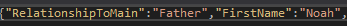
\includegraphics[width=0.8\textwidth]{images/implementation/familyArrayData.png}
    \caption{Screenshot of familyArray file containing correct data}
    \label{fig:implementation-familyArrayData}
\end{figure}
\noindent As I was creating more of the constructor methods, I realised that it would make more sense to move the random generation functions into the \verb|Person| class so that all of the subclasses can use them for their own character generation. The code now looks like this
\begin{lstlisting}[language=c, style=csharp, caption=Random name generation functions]
 //functions used in constructors
public static string genLN()
{
    //Generate female first name
    Random rnd = new Random();
    string[] name = { "Smith", "Brown", "Wilson", "Thomson", "Robertson", "Campbell", "Stewart", "Macdonald", "Murray", "Reid", "Taylor", "Clark", "Mitchell", "Ross", "Watson", "Miller", "Gray", "Simpson", "Duncan", "Bell", "Grant", "Mackenzie", "Allan", "Wood", "Muir", "Watt", "King", "Bruce", "Boyle", "Douglas" };
    string returnName = name[rnd.Next(1, 29)];
    return returnName;
}
public static string genMFN()
{
    //generate male first name
    Random rnd = new Random();
    string[] name = { "Liam", "Noah", "Oliver", "Elijah", "William", "James", "Benjamin", "Ben", "Lucas", "Henry", "Alex", "Ethan", "Daniel", "Sebstian", "Jack", "Matt", "John", "Joe", "David", "Josh", "Julien", "Leo", "Isaac", "Thomas", "Max", "Andy", "Phill", "Harvey", "Ryan" };
    string returnName = name[rnd.Next(1, 29)];
    return returnName;
}

public static string genFFN()
{
    //Generate female first name
    Random rnd = new Random();
    string[] name = { "Olivia", "Sophia", "Maria", "Mia", "Evelyn", "Jess", "Ella", "Zoe", "Jemma", "Gemma", "Emily", "Nuala", "Maggie", "Ciara", "Scarlett", "Layla", "Chloe", "Ellie", "Hazel", "Lucy", "Niamh", "Kat", "Victoria", "Lily", "Hannah", "Chloe", "Lara", "Bella", "Ruby" };
    string returnName = name[rnd.Next(1, 29)];
    return returnName;
}
\end{lstlisting}
I then tested opening a saved game and got an error as the JSON deserialize function creates new instances of the \verb|GenericFamilyMember| to populate as it reads in the file. To fix this, I moved the constructor into a separate method within the \verb|GenericFamilyMember| class and called it like this (shown from the new game form)
\begin{lstlisting}[language=c, style=csharp, caption=Code used to generate generic family members]
for (int i = 0; i < controlClass.NumberOfFamily; i++)
{
    GenericFamilyMember tempFamily = new GenericFamilyMember(); //make new instance of the object
    tempFamily.populateGenericFamilyMember(i, mainCharacter); //populate that object using the 'constructor' in the GenericFamilyMemberclass
    familyArray[i] = tempFamily; //transfer the temp object into the array.
}
\end{lstlisting}

\noindent I then moved onto the generation of the date of birth. To do this, I wrote the following function, which produces a date between 16 and 30 years ago. 
\begin{lstlisting}[language=c, style=csharp, caption=Function which generates DoB of parent]
static DateTime genParentAge(DateTime mcDOB)
{
    //need to generate a date between 16 and 30 years ago from main character birthday.
    DateTime dateOfBirth;
    Random rand = new Random();
    int randomNumber = rand.Next(5845, 10957);
    dateOfBirth = mcDOB.AddDays(-randomNumber);


    return dateOfBirth;
}
\end{lstlisting}
When I tested it, I got the following result; proving it works.
\begin{figure}[H]
    \centering
    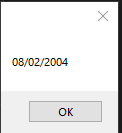
\includegraphics[width=0.3\textwidth]{images/implementation/proofParentAgeGenWorks.png}
    \caption{Proof that the parent DoB generation algorithm works}
    \label{fig:implementation-proofParentAgeGenWorks}
\end{figure}
\noindent As this is working for the father, I implemented it for the mother as well.\\
I then implemented the age calculation algorithm, I thought about a number of different ways I could do this and settled on passing in the character's birthday and returning an integer containing their age.
\begin{lstlisting}[language=c, style=csharp, caption=Age generation algorithm]
public int calcAge(DateTime input)
{
    int difference = (DateTime.Today.Date - input.Date).Days;
    float toround = (difference / 365);
    int age = ((int)toround);

    return age;
}
\end{lstlisting}
This worked first time so I implemented it for the mother as well.\\
The age was the last element I had to programmatically generate for the main character's parents. The finished constructor for the mum and dad can be seen below:
\begin{lstlisting}[language=c, style=csharp, caption=Final code for generation of mother and father to main character]
public GenericFamilyMember populateGenericFamilyMember(int charNumber, MainCharacter mainCharacter)
{
    //construct here
    //go through a swtich statement to set the character based on what their relationship to the main is.
    //setup random number generation
    Random rnd = new Random();
    GenericFamilyMember familyMember = new GenericFamilyMember();
    switch (charNumber)
    {
        case 0:
            //Dad to main character
            RelationshipToMain = "Father";
            FirstName = genMFN();
            LastName = mainCharacter.LastName;
            Gender = "Male";
            Sexuality = "Straight";
            DateOfBirth = genParentAge(mainCharacter.DateOfBirth);
            LivingStatus = true;
            InRelationship = true;
            Age = calcAge(DateOfBirth);
            break;
        case 1:
            //mum to main character
            RelationshipToMain = "Mother";
            FirstName = genFFN();
            switch (rnd.Next(1, 3))
            {
                case 1:
                    //same last name as father and main character
                    LastName = mainCharacter.LastName;
                    break;
                case 2:
                default:
                    //different last name to father and main character - need to randomGen this
                    LastName = genLN();
                    break;
            }
            Gender = "Female";
            Sexuality = "Straight";
            DateOfBirth = genParentAge(mainCharacter.DateOfBirth);
            LivingStatus = true;
            InRelationship = true;
            Age = calcAge(DateOfBirth);
            break;
        default:
            FirstName = null;
            break;
    }
    return familyMember;
}
\end{lstlisting}
While generating a new family member, I received an index out of bounds error for the random name generation. To fix this, I change the top random number to 30 as I had forgotten that arrays are zero-based therefore they don't actually have an item 30 therefore the random generation top bound would need to be reduced by 1. I also moved the random generation lower bound down to 0, to accommodate for the zero-based nature of the array.

\section{Family Tab}
Now I have developed the generation of the various characters, I need a way to display them. I am using the \verb|DataGridView| control which presents the data in table. I did some research and found the following line of code which works and displays the following.
\begin{lstlisting}[language=c, style=csharp, caption=First attempt at using a DataGridView control to show the family tab.]
dgvFamily.DataSource = familyArray;
\end{lstlisting}
\begin{figure}[H]
    \centering
    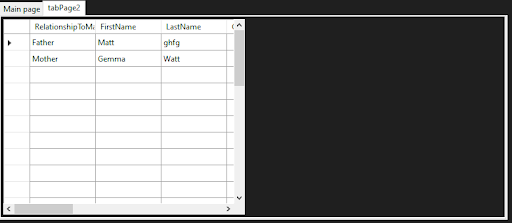
\includegraphics[width=0.8\textwidth]{images/implementation/familyTabInitialTest.png}
    \caption{Result of initial test of using the DataGridView control for the family tab.}
    \label{fig:implementation-familyTabInitialTest}
\end{figure}
\noindent This displays the whole object at once - meaning the user has to scroll horizontally to see all the data. This is not what I wanted so I went back through my old projects and found the code that did what I wanted.
\begin{lstlisting}[language=c, style=csharp, caption=Improved method of populating dgvFamily]
 //first, set var for which column contains which data
int relationshipCol = 0;
int firstNameCol = 1;
int lastNameCol = 2;

//now loop through familyArray and populate dgvFamily
// can use a for loop as number of family members are in the controlClass

for(int x=0; x<controlClass.NumberOfFamily; x++)
{
    int i = dgvFamily.Rows.Add();
    dgvFamily.Rows[i].Cells[relationshipCol].Value = familyArray[x].RelationshipToMain;
    dgvFamily.Rows[i].Cells[firstNameCol].Value = familyArray[x].FirstName;
    dgvFamily.Rows[i].Cells[lastNameCol].Value = familyArray[x].LastName;
}
\end{lstlisting}
This gave me an error: \inlineCode{System.InvalidOperationException: 'Rows cannot be programmatically added to the DataGridView's rows collection when the control is data-bound.'}\\
Which I rectified by removing the previous line of code used by commenting it out. This worked and gave me the result I expected. (At this point, I had also added some colors to the control using Visual Studio's property panel).
\begin{figure}[H]
    \centering
    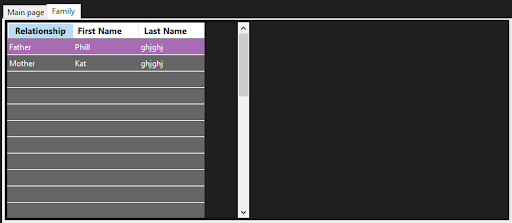
\includegraphics[width=0.8\textwidth]{images/implementation/familyTabSecondTest.png}
    \caption{Second test of displaying information on the DataGridView control}
    \label{fig:implementation-familyTabSecondTest}
\end{figure}
\noindent Now I have the basic code working, I want to change it so it only shows the entries in the array which have data in them. I will do this by including an IF statement inside the FOR loop, like so:
\begin{lstlisting}[language=c, style=csharp, caption=Improved code for displaying data in the DataGridView]
for(int x=0; x<controlClass.NumberOfFamily; x++)
{
    if (familyArray[x].FirstName != null)
    {
        int i = dgvFamily.Rows.Add();
        dgvFamily.Rows[i].Cells[relationshipCol].Value = familyArray[x].RelationshipToMain;
        dgvFamily.Rows[i].Cells[firstNameCol].Value = familyArray[x].FirstName;
        dgvFamily.Rows[i].Cells[lastNameCol].Value = familyArray[x].LastName;
    }
}
\end{lstlisting}
This works and the DataGridView now looks like this:
\begin{figure}[H]
    \centering
    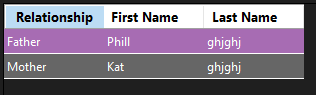
\includegraphics[width=0.4\textwidth]{images/implementation/familyTabFinalDGVTest.png}
    \caption{The DataGridView showing populated rows only}
    \label{fig:implementation-familyTabFinalDGVTest}
\end{figure}
\noindent I then added the code which populates the label controls on the form - this allows the person's information to be displayed to the player.
\begin{lstlisting}[language=c, style=csharp, caption=Code to populate labels on Family Tab containing information about the selected person]
private void dgvFamily_CellContentClick(object sender, DataGridViewCellEventArgs e)
{
   // MessageBox.Show(dgvFamily.CurrentCell.RowIndex.ToString());
    int currentIndex = dgvFamily.CurrentCell.RowIndex;
    //MessageBox.Show(familyArray[currentIndex].Age.ToString());

    //populate info on form
    lblFamRealtionshipToMain.Text = mainCharacter.FirstName + "'s " + familyArray[currentIndex].RelationshipToMain;
    lblFamFirstName.Text = "First Name: " + familyArray[currentIndex].FirstName;
    lblFamLastName.Text = "Last Name: " + familyArray[currentIndex].LastName;
    lblFamGender.Text = "Gender: " + familyArray[currentIndex].Gender;
    lblFamSexuality.Text = "Sexuality: " + familyArray[currentIndex].Sexuality;
    lblFamAge.Text = "Age: " + familyArray[currentIndex].Age.ToString();
    lblFamLivingStatus.Text = "Living Status: " + familyArray[currentIndex].LivingStatus.ToString();
    lblFamDateOfBirth.Text = "Date Of Birth: " + familyArray[currentIndex].DateOfBirth.ToShortDateString();
    lblFamInRelationship.Text = "In Relationship: " + familyArray[currentIndex].InRelationship.ToString();
    if(familyArray[currentIndex].LivingStatus == false)
    {
        //person is dead so can show death date and reason for death
        lblFamDateOfDeath.Text = "Date Of Death: " + familyArray[currentIndex].DateOfDeath.ToShortDateString();
        lblFamReasonForDeath.Text = "Reason For Death: " + familyArray[currentIndex].ReasonForDeath;
    }
    else
    {
        //person is not dead - don't show death date and reason for death
        lblFamDateOfDeath.Text = "Date Of Death: N/A (haven't died yet!)";
        lblFamReasonForDeath.Text = "Reason For Death: N/A (haven't died yet!)";
    }
}
\end{lstlisting}
\begin{figure}[H]
    \centering
    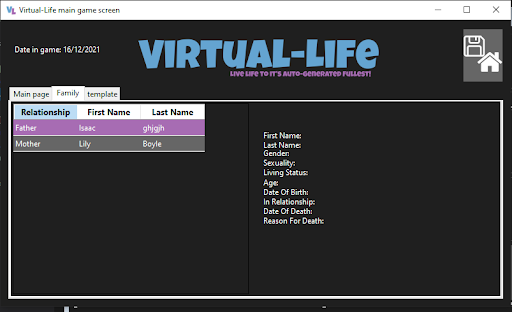
\includegraphics[width=0.8\textwidth]{images/implementation/familyTabLabelsPre.png}
    \caption{Empty labels, before any information is put into them}
    \label{fig:implementation-familyTabLabelsPre}
\end{figure}
\begin{figure}[H]
    \centering
    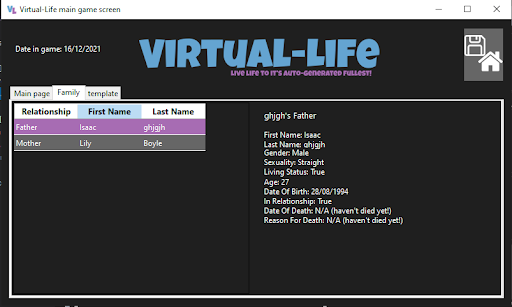
\includegraphics[width=0.8\textwidth]{images/implementation/familyTabLabelsPost.png}
    \caption{Filled out labels, after the father has been selected}
    \label{fig:implementation-familyTabLabelsPost}
\end{figure}
\noindent In the figures above, it looks like the father has been selected before it actually has. This is a feature of the \verb|DataGridView|, in that there has to be a row \textquotesingle selected\textquotesingle  at all times.

\section{Loading the Files in}
During developmental testing, I realised that I had quite a serious bug. From moving from system to system, the filepath of the game wasn't dynamically adapting to the system, meaning I couldn't use a save I made on the college computer at home as the file path in the control class was wrong. To resolve this issue, I added this line of code to the opening files form:
\begin{lstlisting}[language=c, style=csharp, caption=Line of code used to fix the filepath issues]
controlClass.Filepath = filepath;
\end{lstlisting}
This overrides whatever had been read in from the control class file with the location specified by the user to find the saved data from the game.

\section{Death}
Now, I need to start processing the events of the age up algorithm, the first thing I am going to program is the death checker. This algorithm will check based on the character\textquotesingle s age the probability of them dying and return a boolean for if they shall live or not, if they don't live, then their data will be sent to another subroutine which will ‘kill' them and update the relevant variables to reflect this. I started by testing the ageing up of family members and realised that I hadn't yet programmed this. This means I have to do this first.\\
I added a procedure in which loops through all the elements of the array \verb|familyArray| and if the living status is true, then it adds 1 to the age of the character. This will allow me to not age up characters once they have died.
\begin{lstlisting}[language=c, style=csharp, caption=Method which increases the age of the family array]
private void ageUpFamilyArray()
{
    //loop through all the members of the family array and add 1 to their age if livingstatus is true
    for(int x=0; x<controlClass.NumberOfFamily; x++)
    {
        if(familyArray[x].LivingStatus == true)
        {
            //can age them up
            familyArray[x].Age = familyArray[x].Age + 1;
        }
    }
}
\end{lstlisting}
To confirm that this was working as intended, I ran the code and confirmed the father of the main characters age before and after I pressed the age up button. It behaved as expected; therefore I was satisfied to move onto the next aspect of the death checker.\\
I added the following code which changes the chance of the main character dying based on their age.
\begin{lstlisting}[language=c, style=csharp, caption=Main character death checker algorithm]
public bool deathCheckerMainCharacter(int age)
{
    bool deathBool = false;
    
    int age = mainCharacter.Age;
    int deathChance = 1;
    //for as main char gets older, their death chance increases
    /* 00-10 1/30 
     * 11-16 1/25
     * 17-30 1/15 
     * 31-50 1/25 
     * 51-67 1/20 
     * 68-80 1/15 
     * 81-100 1/8 
     * >100 1/3 
     */
    if (age <= 10)
    {
        deathChance = 30;
    }
    else if (age >= 11 && age <= 16)
    {
        deathChance = 25;
    }
    else if (age >= 17 && age <= 30)
    {
        deathChance = 15;
    }
    else if (age >= 31 && age <= 50)
    {
        deathChance = 25;
    }
    else if (age >= 51 && age <= 67)
    {
        deathChance = 20;
    }
    else if (age >= 68 && age <= 80)
    {
        deathChance = 15;
    }
    else if (age >= 81 && age <= 99)
    {
        deathChance = 8;
    }
    else if (age >= 100)
    {
        deathChance = 3;
    }
    //now generate random number based off of 1 and deathChance
    Random rnd = new Random();
    int randomReturn = rnd.Next(1, deathChance);
    if (randomReturn == 2)
    {
        //DEATH
        deathBool = true;
    }
    else
    {
        deathBool = false;
    }

    //return deathBool to main program where it will be processed.
    return deathBool;
}
\end{lstlisting}
I then added the code which will programmatically kill the main character:
\begin{lstlisting}[language=c, style=csharp, caption=Kill main character method]
public void killMainCharacter()
{
    //very rough for now, will need to polish at some point

    btnAgeUp.Enabled = false;
    mainCharacter.DateOfDeath = controlClass.InGameDate; 
    mainCharacter.LivingStatus = false;
    mainCharacter.ReasonForDeath = generateReasonForDeath();
    //generate event showing this
    eventArray[controlClass.NextEvent].Category = "Death";
    eventArray[controlClass.NextEvent].DateHappened = controlClass.InGameDate;
    eventArray[controlClass.NextEvent].Description = "You died due to " + mainCharacter.ReasonForDeath;
    controlClass.NextEvent++;
    MessageBox.Show(mainCharacter.FirstName + " has died a tragic death due to " + mainCharacter.ReasonForDeath, mainCharacter.FirstName + " has died", MessageBoxButtons.OK, MessageBoxIcon.Exclamation);
    saveToFile();
}
\end{lstlisting}
This produces the outcome of:
\begin{figure}[H]
    \centering
    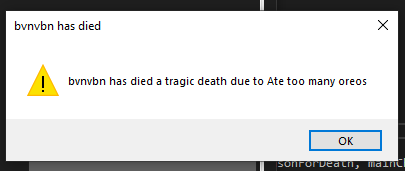
\includegraphics[width=0.5\textwidth]{images/implementation/deathProof1.png}
    \caption{Alerting message box displayed when Main Character Dies}
    \label{fig:implementation-deathProof1}
\end{figure}
\begin{figure}[H]
    \centering
    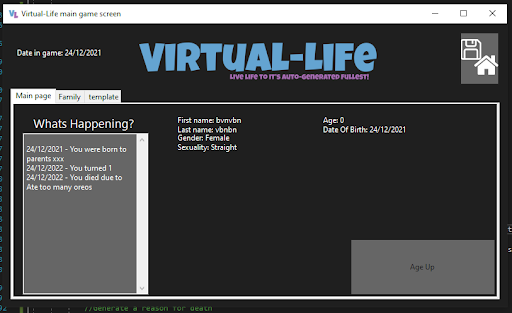
\includegraphics[width=0.8\textwidth]{images/implementation/deathProof2.png}
    \caption{Main game screen showing death event and age up button disabled}
    \label{fig:implementation-deathProof2}
\end{figure}
\noindent I then moved onto the killing algorithm of the other characters, this will be done in a similar way to the increasing age of them - looping through the array and if they aren't already dead then passing them through the death checker then if they are to die, passing them through a kill procedure which will make use of the same \verb|generateReasonForDeath| function.
This was very easy to program as I had already worked out the fundamentals of this in the main character killing functions, so I was able to copy, paste and adapt the code to suit the \verb|genericFamilyMember| objects.
\begin{lstlisting}[language=c, style=csharp, caption=Death algorithm for a non-main character]
public void checkKillGenericFamilyMember()
{
    //loop through all members of familyArray, passing their age into deathCheck. if return=true then kill, else move onto next.

    for(int x=0; x<controlClass.NextFamily; x++)
    {
        if(familyArray[x].LivingStatus == true)
        {
            bool deathCheckReturn = deathCheck(familyArray[x].Age);
            if(deathCheckReturn == true)
            {
                //RIP - put death code here
                //MessageBox.Show("DEATH" + x.ToString());
                familyArray[x].DateOfDeath = controlClass.InGameDate.AddDays(randomNumber(1, 300));
                familyArray[x].LivingStatus = false;
                familyArray[x].ReasonForDeath = generateReasonForDeath();
                //Now gen event
                eventArray[controlClass.NextEvent].Category = "Death";
                eventArray[controlClass.NextEvent].DateHappened = controlClass.InGameDate;
                eventArray[controlClass.NextEvent].Description = familyArray[x].FirstName + " (your " + familyArray[x].RelationshipToMain.ToLower() + ") died due to " + familyArray[x].ReasonForDeath;
                controlClass.NextEvent++;
                //now reduce mc happiness score
                mainCharacterScores.HappinessScore = mainCharacterScores.HappinessScore - randomNumber(1, 100);
                saveToFile();
            }
        }
    }
}
\end{lstlisting}
For the purposes of testing, I added in a line of code which will force the character to die. This is omitted from the code above.\\
\begin{figure}[H]
    \centering
    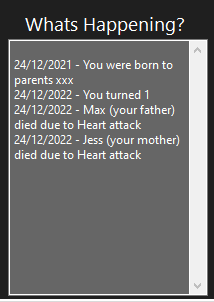
\includegraphics[width=0.3\textwidth]{images/implementation/deathProofGeneric.png}
    \caption{Event box on main game screen showing someone has died}
    \label{fig:implementation-deathProofGeneric}
\end{figure}
I then included more reasons for death. My reasons for death array now contains the following:
\begin{lstlisting}[language=c, style=csharp, caption=Reasons for death array]
string[] reasonsForDeath = { "a heart attack", "eating too many oreos", "being clawed at by cat" , "slipping on a banana peel", "falling in the otter enclosure at a zoo and being licked to death", "dropping a toaster into the bath", "being crushed by a falling grand piano", "being strangled by a fez tassel", "walking into a cactus", "getting hit by a train", "being clubbed by old lady in the street with her walker", "being crushed by a stampede of hungry campers"};
\end{lstlisting}

\section{Random Generation Of a Main Character}
At this point in developmental testing, I was creating a new game relatively frequently, to allow me to test different aspects. It takes about a minute to setup the main character in the new game form, even with just entering gobbledygook. To improve on this time, I created a random generation button with the following code behind it.
\begin{lstlisting}[language=c, style=csharp, caption=Random generation of main character algorithm]
private void btnRandom_Click(object sender, EventArgs e)
{
    Random rnd = new Random();
    int gender = rnd.Next(1, 3);
    switch (gender)
    {
        case 1:
            //male
            txtFirstName.Text = Person.genMFN();
            cboGender.Text = "Male";
            break;
        case 2:
            //female
            txtFirstName.Text = Person.genFFN();
            cboGender.Text = "Female";
            break;
        default:
            txtFirstName.Text = "Sam";
            break;
    }
    txtLastName.Text = Person.genLN();
    int hair = rnd.Next(1,5);
    int eye = rnd.Next(1, 6);

    switch (hair)
    {
        case 1:
            cboHairColour.Text = "Blonde";
            break;
        case 2:
            cboHairColour.Text = "Brown";
            break;
        case 3:
            cboHairColour.Text = "Red";
            break;
        case 4:
            cboHairColour.Text = "Black";
            break;
        default:
            cboHairColour.Text = "Blonde";
            break;
    }

    switch (eye)
    {
        case 1:
            cboEyeColour.Text = "Brown";
            break;
        case 2:
            cboEyeColour.Text = "Blue";
            break;
        case 3:
            cboEyeColour.Text = "Green";
            break;
        case 4:
            cboEyeColour.Text = "Gray";
            break;
        case 5:
            cboEyeColour.Text = "Amber";
            break;
        default:
            cboEyeColour.Text = "Brown";
            break;
    }
    
}
\end{lstlisting}
This works as expected and produces a random character.

\section{Scores}
Before I programmed any more of the game, I decided that I would need to add in the code for my scores. I first added the \verb|Score| class.
\begin{lstlisting}[language=c, style=csharp, caption=Score class]
public class Score
{
    private int educationScore;
    private int jobScore;
    private int happinessScore;
    private int medicalScore;
    private int lifeScore;

    public int EducationScore { get; set; }
    public int JobScore { get; set; }
    public int HappinessScore { get; set; }
    public int MedicalScore { get; set; }
    public int LifeScore { get; set; }
}
\end{lstlisting}
I then added the code to the constructor of the create new game form which will create a new object called \verb|mainCharacterScores|.
\begin{lstlisting}[language=c, style=csharp, caption=Declaration of the mainCharacterScores object]
public Score mainCharacterScores = new Score();
\end{lstlisting}
I then added the the initialisation code with placeholder values.
\begin{lstlisting}[language=c, style=csharp, caption=Setting the score values to placeholder values]
//setup the scores object for the main (use random generation to calculate values)
mainCharacterScores.EducationScore = 0;
mainCharacterScores.JobScore = 0;
mainCharacterScores.HappinessScore = 0;
mainCharacterScores.MedicalScore = 0;
mainCharacterScores.LifeScore = 0;
\end{lstlisting}
Now, I need to add the code to write this new object out to a file (on the \verb|MainGameScreen| form)
\begin{lstlisting}[language=c, style=csharp, caption=Code to write the Scores object out to a file]
File.WriteAllText(controlClass.Filepath + "\\mainCharacterScores.json", JsonConvert.SerializeObject(mainCharacterScores));
\end{lstlisting}
To test this first, I created a new game then saved it and viewed the \verb|mainCharacterScores.Json| file in Notepad++. I saw what I was expecting
\begin{figure}[H]
    \centering
    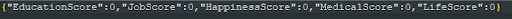
\includegraphics[width=0.8\textwidth]{images/implementation/scoresTest1.png}
    \caption{Screenshot of Notepad++ showing scores object}
    \label{fig:implementation-scoresTest1}
\end{figure}
\noindent Now I can write the data out to a file, I need a way to read it back into the game. I added the code needed in the show saved games form for this.
\begin{lstlisting}[language=c, style=csharp, caption=Code to read mainCharacterScores back in]
Score mainCharacterScores = JsonConvert.DeserializeObject<Score>(File.ReadAllText(filepath + "\\mainCharacterScores.json"));
\end{lstlisting}
I then added the code in to show the life score in a message box, so I could test opening the same saved game files.
\begin{lstlisting}[language=c, style=csharp, caption=Test code to make sure code above is working]
MessageBox.Show(mainCharacterScores.LifeScore.ToString());
\end{lstlisting}
This worked as expected and produced the following result
\begin{figure}[H]
    \centering
    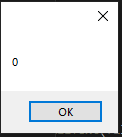
\includegraphics[width=0.2\textwidth]{images/implementation/scoresTest2.png}
    \caption{Proof the scores are being read back into the program correctly}
    \label{fig:implementation-scoresTest2}
\end{figure}
\noindent I then removed the code for the message box because now that I know that the file management is working, I can now add in the algorithms for all these values and the displays in the game window for them. To start, I will add in the code to the create new game form to randomly generate the initial score values. I will be using an instance of the \verb|Random| class called \verb|rnd| to generate the scores. Each score will have a maximum value of 100.
\begin{lstlisting}[language=c, style=csharp, caption=Setting the score values random values]
//setup the scores object for the main (use random generation to calculate values)
mainCharacterScores.EducationScore = rnd.Next(0, 101);
mainCharacterScores.JobScore = rnd.Next(0, 101);
mainCharacterScores.HappinessScore = rnd.Next(0, 101);
mainCharacterScores.MedicalScore = rnd.Next(0, 101);
mainCharacterScores.LifeScore = rnd.Next(0, 101);
\end{lstlisting}
To display this information, I will take inspiration from one of the games which I was playing during research - using a bar to represent the information. I will use the control ProgressBar as they are easy to set the value of and a nice visual representation of the value.
\begin{figure}[H]
    \centering
    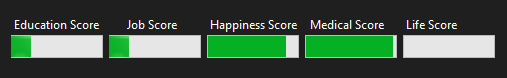
\includegraphics[width=0.8\textwidth]{images/implementation/scoresTest3.png}
    \caption{Progress bar controls containing the score values}
    \label{fig:implementation-scoresTest3}
\end{figure}
\noindent (Colours and placement are subject to redesign)\\
I then added the code to make each of the progress bars fill depending on the value of the score.
\begin{lstlisting}[language=c, style=csharp, caption=Code to display the score in the progress bar]
public void updateScoresPB()
{
    prbEducationScore.Value = mainCharacterScores.EducationScore;
    prbJobScore.Value = mainCharacterScores.JobScore;
    prbHappinessScore.Value = mainCharacterScores.HappinessScore;
    prbMedicalScore.Value = mainCharacterScores.MedicalScore;
    prbLifeScore.Value = mainCharacterScores.LifeScore;
}
\end{lstlisting}
As with most of my program, I am breaking it down into smaller functions or procedures as I will need to use the code in many different places.

\section{Education}
Now I have my scores and displaying of said scores working, I can begin writing the code which will alter the scores. The first score I will program is the education score. To start off, I setup the code which will calculate the next 1st September based off of the character's date of birth then work out what year they should be moving into in school.
\begin{lstlisting}[language=c, style=csharp, caption=Procedure to check the education status of the main character]
public void checkEducationStatus()
{
    int age = mainCharacter.Age;
    DateTime mcBirthday = mainCharacter.DateOfBirth;
    DateTime dateOfEvent;
    if (mcBirthday.DayOfYear < 245)
    {
        //mc is born before 2nd sept therefor events need to be for this september
        int yearOfEvent = controlClass.InGameDate.Year;
        int monthOfEvent = 9;
        int dayOfEvent = 1;
        dateOfEvent = new DateTime(yearOfEvent, monthOfEvent, dayOfEvent);
    }
    else
    {
        //mc is born after 2nd sept therfore events need to be for the following september
        int yearOfEvent = (controlClass.InGameDate.Year) + 1;
        int monthOfEvent = 9;
        int dayOfEvent = 1;
        dateOfEvent = new DateTime(yearOfEvent, monthOfEvent, dayOfEvent);
    }
    //need to get date of 1st september after mcs birthday
    switch (age)
    {
        case 4:
            //move into reception
            eventArray[controlClass.NextEvent].Category = "Education";
            eventArray[controlClass.NextEvent].DateHappened = dateOfEvent;
            eventArray[controlClass.NextEvent].Description = "Move into year 4";
            controlClass.NextEvent++;
            break;
\end{lstlisting}
For testing, I have just used the first year - age 4 where the character will be entering reception. The test code I wrote works and displays the following. Where it says  'move into year4', this should read 'move into reception'. This is not an program error, this is a typing error on my part.
\begin{figure}[H]
    \centering
    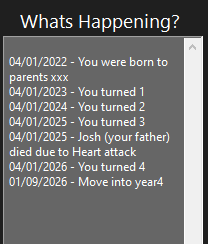
\includegraphics[width=0.3\textwidth]{images/implementation/educationTest1.png}
    \caption{Event box showing first school event}
    \label{fig:implementation-educationTest1}
\end{figure}
\noindent I then setup the page of the TabControl which will display the education information. It is basic for the moment, this may be improved at a later point.
\begin{figure}[H]
    \centering
    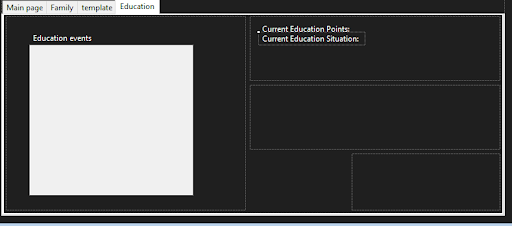
\includegraphics[width=0.8\textwidth]{images/implementation/educationTest2.png}
    \caption{TabControl showing education page}
    \label{fig:implementation-educationTest2}
\end{figure}
\noindent Now, I will add the code to populate the form.
\begin{lstlisting}[language=c, style=csharp, caption=Code to populate the education page on the main game form]
public void updateEducationPage()
{
    //first update the events box
    txtEduEducationEvents.ResetText();
    for (int i = 0; i < controlClass.NextEvent; i++)
    {
        if(eventArray[i].Category == "Education")
        {
            txtEduEducationEvents.Text = txtEduEducationEvents.Text + Environment.NewLine + eventArray[i].DateHappened.ToShortDateString() + " - " + eventArray[i].Description;
        }
        
    }

    //now update the lables
    lblEduCurrentEducationPoints.Text = "Current Education Points: " + mainCharacterScores.EducationScore.ToString();
    lblEduEducationSituation.Text = "Current Education Situation: At school - " + controlClass.NameOfCurrentSchool;
    lblEduCurrentYear.Text = "Current Year: " + controlClass.CurrentSchoolYear.ToString();
}
\end{lstlisting}
Which will produce the following result, again please ignore the typo in the 'move into year4' line.
\begin{figure}[H]
    \centering
    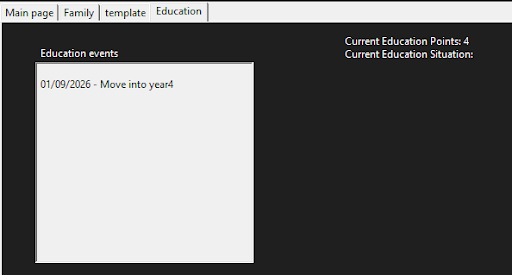
\includegraphics[width=0.8\textwidth]{images/implementation/educationTest3.png}
    \caption{Populated education page on main form}
    \label{fig:implementation-educationTest3}
\end{figure}
\noindent Now, I have the basics working, I need to go through each of the years and add in the events. These will be hard coded for now to save time. If I get more time, I will add in some customisation for this from the players perspective.\\
Shown below is the code for each age of the character. Only shown below is for when the character is 4.
\begin{lstlisting}[language=c, style=csharp, caption=First improvement to the education generation procedure]
case 4:
    //move into reception
    eventArray[controlClass.NextEvent].Category = "Education";
    eventArray[controlClass.NextEvent].DateHappened = dateOfEvent;
    eventArray[controlClass.NextEvent].Description = "Start infant school in Reception.";
    controlClass.NextEvent++;
    mainCharacterScores.EducationScore = mainCharactedScores.EducationScore + randomNumber (1,4);
    break;
\end{lstlisting}

\begin{figure}[H]
    \centering
    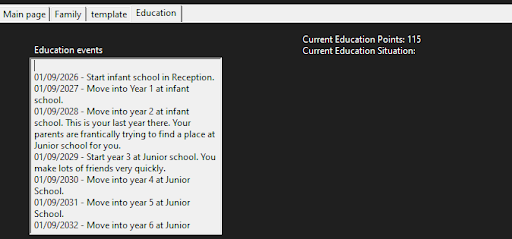
\includegraphics[width=0.8\textwidth]{images/implementation/educationTest4.png}
    \caption{Output of the first improvement of the education system}
    \label{fig:implementation-educationTest4}
\end{figure}
\noindent I got an error during testing where the score value was greater than the max value of the progress bar. This is caused by the progress bar control which displays the education score having a maximum value of 100, and the education score value being set to 101 in the code.\\
To resolve this, I added in an if statement to the update progress bars method.
\begin{lstlisting}[language=c, style=csharp, caption=Improved updateScoresPB procedure]
public void updateScoresPB()
{
    if (mainCharacterScores.EducationScore < prbEducationScore.Maximum && mainCharacterScores.EducationScore > prbEducationScore.Minimum)
    {
        prbEducationScore.Value = mainCharacterScores.EducationScore;
    }
    if(mainCharacterScores.HappinessScore < prbHappinessScore.Maximum && mainCharacterScores.HappinessScore > prbHappinessScore.Minimum)
    {
        prbHappinessScore.Value = mainCharacterScores.HappinessScore;
    }
    if (mainCharacterScores.MedicalScore < prbMedicalScore.Maximum && mainCharacterScores.MedicalScore > prbMedicalScore.Minimum)
    {
        prbMedicalScore.Value = mainCharacterScores.MedicalScore;
    }
    if (mainCharacterScores.LifeScore < prbLifeScore.Maximum && mainCharacterScores.LifeScore > prbLifeScore.Minimum)
    {
        prbLifeScore.Value = mainCharacterScores.LifeScore;
    }
}
\end{lstlisting}
This only updates the progress bar if the education score is less than the maximum value and greater than the minimum value of the progress bar.\\
To progress further with the education generation, I need to now program the choice box form. This will allow the user to select one of three pre-determined options on a new form.

\section{Choice Box Form}
I began by designing the form. All the label controls will be populated programmatically as part of the construction of the form when it is needed; this is why they have been left as the default placeholder text.
\begin{figure}[H]
    \centering
    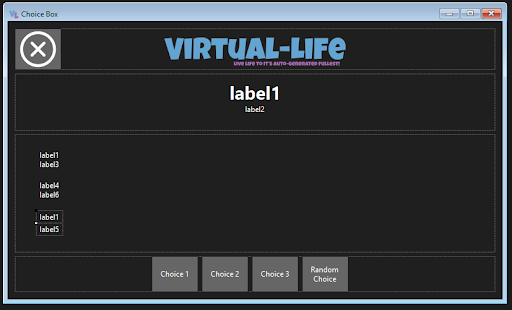
\includegraphics[width=0.8\textwidth]{images/implementation/choiceBox1.png}
    \caption{Choice Box form design}
    \label{fig:implementation-choiceBox1}
\end{figure}
\noindent
Now, I will add the code to pass some test data into the form from my test button on the main game form. Below is the code on \verb|frmMainGameScreen| which calls the choice box.
\begin{lstlisting}[language=c, style=csharp, caption=Code which generates the choice box form and recieves its response]
using (var form = new frmChoiceBox("text here"))
{
    var result = form.ShowDialog();
    if (result == DialogResult.OK)
    {
        string val = form.ReturnValue1; //values preserved after close
        //Do something here with these values
        MessageBox.show(val);
    }
}
\end{lstlisting}
Below is the code on the choice box form which responds to the user pressing \verb|btnChoice1|.
\begin{lstlisting}[language=c, style=csharp, caption=Choice box form code to send the result to where it was called from]
public partial class frmChoiceBox : Form
{
    public string ReturnValue1{get; set; }
    string headerHere;
    public fromChoiceBox(string header)
    {
        InitializeComponent();
        headerHere = header;
    }
    
    private void frmChoiceBox_Load(object sender, EventArgs e)
    {
        MessageBox.show(headerHere);
    }
    
    private void btnChoice1_Click(object sender, EventArgs e)
    {
        this.ReturnValue1 = "Something";
        this.DialogResult = DialogResult.OK;
        this.Close();
    }
}
\end{lstlisting}
When running this, I will expect to see a message box containing "Text here", then the form will appear. When I click the \verb|btnChoice1|, I expect the form to close then a message box to appear containing the word "something".\\
I will now run the program and check what happens.
\noindent First, this message box appears
\begin{figure}[H]
    \centering
    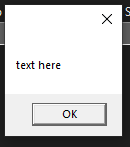
\includegraphics[width=0.3\textwidth]{images/implementation/choiceBox2a.png}
    \caption{Testing choice box 1a}
    \label{fig:implementation-choiceBox2a}
\end{figure}
\noindent Then the form appears
\begin{figure}[H]
    \centering
    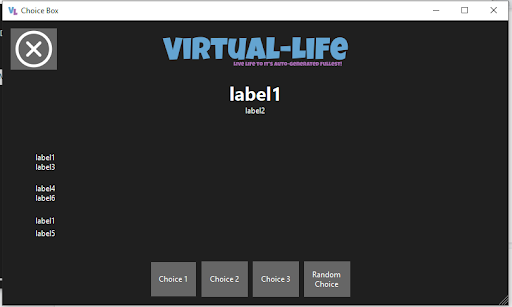
\includegraphics[width=0.8\textwidth]{images/implementation/choiceBox2b.png}
    \caption{Testing choice box 1b}
    \label{fig:implementation-choiceBox2b}
\end{figure}
\noindent Then when I click choice 1, the form closes then this message box appears.
\begin{figure}[H]
    \centering
    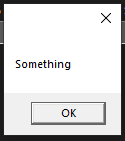
\includegraphics[width=0.3\textwidth]{images/implementation/choiceBox2c.png}
    \caption{Testing choice box 1c}
    \label{fig:implementation-choiceBox2c}
\end{figure}
\noindent This means that this code is working and I can progress onto adding more data passed into the form's constructor.\\
First though, I need to stop the user from selecting anything on the \verb|mainGameScreen| form while the choice box is active. I could either disable all the controls on it or I could just hide the form then re-show it when it\textquotesingle s needed. I'm going to use the latter. To test this, I added in the code to hide the main game form once it had loaded the choice form, then when a response is received from the choice form, re-show the main form.
\begin{lstlisting}[language=c, style=csharp, caption=Code which generates the choice box form and receives its response now with show and hide functions]
using (var form = new frmChoiceBox("text here"))
{
    this.Hide();
    var result = form.ShowDialog();
    this.Show();
    if (result == DialogResult.OK)
    {
        string val = form.ReturnValue1; //values preserved after close
        //Do something here with these values
        MessageBox.show(val);
    }
}
\end{lstlisting}
Now, I need to write the constructor function which will generate the box and process the box. I am writing it this way as I will potentially need to use this form multiple times in one game, meaning I will need to have a reusable piece of code which can be used to generate it.
I added the code needed to send text into and return a value from the choice box. I am expecting a message box to show containing 556 when I close out of the choice box.
\begin{figure}[H]
    \centering
    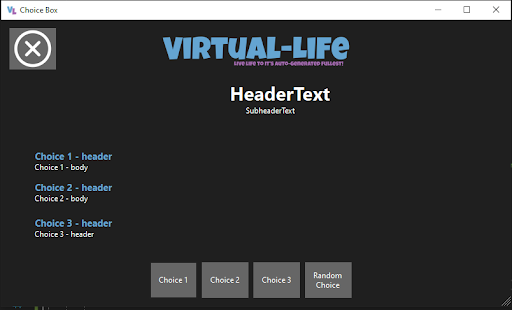
\includegraphics[width=0.8\textwidth]{images/implementation/choiceBox3a.png}
    \caption{Form with data passed into it programmatically}
    \label{fig:implementation-choiceBox3a}
\end{figure}
\begin{figure}[H]
    \centering
    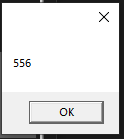
\includegraphics[width=0.3\textwidth]{images/implementation/choiceBox3b.png}
    \caption{Result of pressing button "Choice 1"}
    \label{fig:implementation-choiceBox3b}
\end{figure}
\noindent This means I have a working choice box, for choice 1 at least.
Now I will program the other 4 buttons and test them. I have written the following code to return the value of the button that the user presses.
\begin{lstlisting}[language=c, style=csharp, caption=Code which returns the outcome of the choice box]
private void btnChoice1_Click(object sender, EventArgs e)
{
    this.ReturnValue1 = 1;
    this.DialogResult = DialogResult.OK;
    this.Close();
    
}

private void btnChoice2_Click(object sender, EventArgs e)
{
    this.ReturnValue1 = 2;
    this.DialogResult = DialogResult.OK;
    this.Close();
}

private void btnChoice3_Click(object sender, EventArgs e)
{
    this.ReturnValue1 = 3;
    this.DialogResult = DialogResult.OK;
    this.Close();
}

private void btnRandomChoice_Click(object sender, EventArgs e)
{
    Random rnd = new Random();
    int random = rnd.Next(1, 4);
    this.ReturnValue1 = random;
    this.DialogResult = DialogResult.OK;
    this.Close();
}

private void button1_Click(object sender, EventArgs e)
{
    this.DialogResult = DialogResult.Cancel;
    this.Close();
}
\end{lstlisting}
This is working as expected.\\
Now I have a working choice box which I can feed data into, I need to use it to make some decisions in the game. I am first going to use it when the character turns 4 and has to decide what school to go to. 

\section{Generating names error}
While generating a new game for testing, I came across a bug which is where I have set the upper bound of a random generation too high for the array it is in. This has been a recurring issues with each of the three name generation functions. 
For example, I have given 31 as the upper bound for an array which contains exactly 30 items, when you take into account the zero based nature of arrays in C\#, the error is generated.\\
To fix this error, I have reduced the upper bound to 29. This is working.

\section{Random Generation of Names of Schools}
Now I have the choice box and education system vaguely worked out. I can begin to randomly generate names of schools.
I added the following code to my program

\begin{lstlisting}[language=c, style=csharp, caption=Random generation of schools code]
public int choiceBox(int typeOfChoice, string opt1, string opt2, string opt3)
{
    /*
     * Will need to pass the following into this function and into the choice box form.
     * -type of choice (this will determine the header and subheader text)
     * --> using this rather than passing all information in to simplifiy calls to this function.
     * -opt1
     * -opt2
     * -opt3
     */

    //declare vars used for passing data to choice box
    string headerText = "HeaderText";
    string subheaderText = "SubheaderText";
    string opt1header = "Choice 1";
    string opt1body = opt1;
    string opt2header = "Choice 2";
    string opt2body = opt2;
    string opt3header = "Choice 3";
    string opt3body = opt3;


    //first setup the typeOfChoice
    switch (typeOfChoice)
    {
        case 1:
            //choose infant school
            headerText = "Infant school";
            subheaderText = "Select the infant school you want to spend the next 3 years at";
            break;
        case 2:
            //choose junior school
            headerText = "Junior school";
            subheaderText = "Select the junior school you want to spend the next 4 years at";
            break;
        case 3:
            //choose secondary school
            headerText = "Secondary school";
            subheaderText = "Select the secondary school you want to spend the next 5 years at";
            break;
        case 4:
            //choose college
            headerText = "College";
            subheaderText = "Select the college you want to spend the next 2 years at";
            break;
        default:
            //no option found
            break;
    }

    using (var form = new frmChoiceBox(headerText, subheaderText, opt1header, opt1body, opt2header, opt2body, opt3header, opt3body))
    {

        this.Hide();
        var result = form.ShowDialog();

        this.Show();
        if (result == DialogResult.OK)
        {
            int val = form.ReturnValue1;            //values preserved after close
            //Do something here with these values

            //for example
            
            return (val);
        }
        
    }
    return 0;
}
\end{lstlisting}
When I ran it for the first time, I got the following output. This is erroneous as there is no option for choice 3.
\begin{figure}[H]
    \centering
    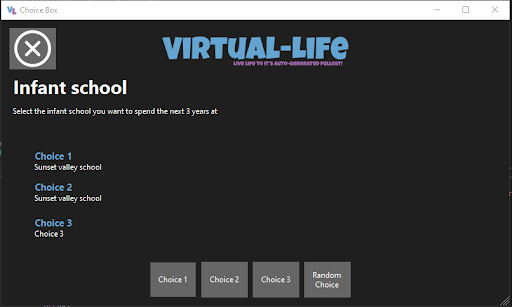
\includegraphics[width=0.8\textwidth]{images/implementation/schoolGen1.png}
    \caption{Output from first run of Random School Generation Code}
    \label{fig:implementation-schoolGen1}
\end{figure}
\noindent I don't mind that choices 1 and 2 are the same as this could add some comedic value to the game.\\
On debugging, I was able to find a typo in the constructor for the choice box form.
\begin{lstlisting}[language=c, style=csharp, caption=Erronious line]
opt3body = opt3h;
\end{lstlisting}
\begin{lstlisting}[language=c, style=csharp, caption=Corrected line]
opt3body = opt3b;
\end{lstlisting}
This correction worked, and I got the result which I was expecting.
\begin{figure}[H]
    \centering
    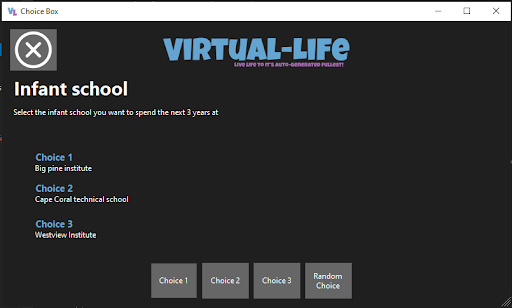
\includegraphics[width=0.8\textwidth]{images/implementation/schoolGen2.png}
    \caption{Correct output from random school name generation code}
    \label{fig:implementation-schoolGen2}
\end{figure}
\noindent Now I have the school name generation worked out for the infant school, I can re-use the functions to generate names of schools for junior and secondary.\\
After adding the code to make this work. I tested this and it works as expected.

\section{Textboxes}
During testing, I was finding it annoying having to scroll down through the events text box and education text box to find the latest event. To solve this, I've changed the code which adds the latest event to the text box from 
\begin{lstlisting}[language=c, style=csharp, caption=Old method of adding text to textbox]
txtEventBox.Text = txtEventBox.Text + Environment.NewLine + eventArray[i].DateHappened.ToShortDateString() + " - " +  eventArray[i].Description;
\end{lstlisting}
to
\begin{lstlisting}[language=c, style=csharp, caption=New method of adding text to a textbox]
txtEventBox.AppendText(Environment.NewLine + eventArray[i].DateHappened.ToShortDateString() + " - " + eventArray[i].Description);
\end{lstlisting}
This has solved my problem and now the textbox scrolls down as the new content is added to it.

\section{Withdraw from Education}
Part of my design is having a way for the character to withdraw from Education.\\
First, I added the button onto the form which will allow this to happen.
\begin{figure}[H]
    \centering
    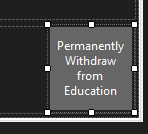
\includegraphics[width=0.2\textwidth]{images/implementation/withdraw1.png}
    \caption{Permanently withdraw from education button}
    \label{fig:implementation-withdraw1}
\end{figure}
\noindent I then added the code to support the button
\begin{lstlisting}[language=c, style=csharp, caption=Withdraw from Education button code]
private void btnEduWithdraw_Click(object sender, EventArgs e)
{
    mainCharacter.InEducation = false;
    eventArray[controlClass.NextEvent].Category = "Education";
    eventArray[controlClass.NextEvent].DateHappened = controlClass.InGameDate;
    eventArray[controlClass.NextEvent].Description = "You permanently withdrew from education. You said it was too boring.";
    controlClass.NextEvent++;
    mainCharacterScores.EducationScore = 0;
}
\end{lstlisting}
I then added an if statement to the checkEducationStatus procedure to check if the character was currently in education or not.\\
This feature works. On the click of age up directly following pressing the withdraw button it gives you the following event:
\begin{figure}[H]
    \centering
    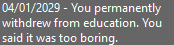
\includegraphics[width=0.2\textwidth]{images/implementation/withdraw2.png}
    \caption{Event generated after pressing Withdraw button}
    \label{fig:implementation-withdraw2}
\end{figure}

\section{Being Born Event}
Currently, when a new game is started, the first event generated states “You were born to parents xxx”. Now I have my parent generation code written, I can add in the parent's names. To do this, I will need to move the code which generates the event from the middle of the new life algorithm to the end, this will make sure that the parents have been generated before their information is inputted to the event array.\\
I also need to change the code which generates the event so it has the names in it.
\begin{lstlisting}[language=c, style=csharp, caption=Improved code for the being born event]
eventArray[controlClass.NextEvent].Category = "Life Event";
eventArray[controlClass.NextEvent].DateHappened = DateTime.Today;
eventArray[controlClass.NextEvent].Description = "You were born to parents " + familyArray[0].FirstName + " and " + familyArray[1].FirstName;
controlClass.NextEvent++;
\end{lstlisting}
This worked the first time I ran the code and gave me the result I was expecting.
\begin{figure}[H]
    \centering
    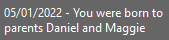
\includegraphics[width=0.2\textwidth]{images/implementation/birthEvent1.png}
    \caption{Event generated after being born}
    \label{fig:implementation-birthEvent1}
\end{figure}

\section{Generate Event Procedure}
It is quite laborious having to write 4 lines of code to generate a single event. As I am using this more and more, I am going to write a procedure which will do it for me.\\
I used my standard 4 lines of code and copied them into a procedure then wrote the test code to test it with.
\begin{lstlisting}[language=c, style=csharp, caption=Code for generateEvent procedure]
public void generateEvent(string category, string content, DateTime date)
{
    eventArray[controlClass.NextEvent].Category = category;
    eventArray[controlClass.NextEvent].DateHappened = date;
    eventArray[controlClass.NextEvent].Description = content;
    controlClass.NextEvent++;
}
\end{lstlisting}
This worked the first time I ran it and produced the result I was expecting.

\section{Scores}
Now I have some of the bigger elements of the game programmed, I can start thinking more about the scores. To do this, I need to generate modifiers; this is where the \verb|ControlClass| will be used to store these modifiers. Then I will be able to write my \verb|lifeScore| algorithm.\\
First, I am going to change how the scores are initially assigned to the character. The character\textquotesingle s job score and education score will start off at zero, as in real life this is how it works. For now, I am also setting the medical score to 0 as I still need to write the algorithm which will calculate this and generate conditions for the characters. Happiness score will still be randomly generated as this is relatively random in life. After making these changes, this is what the declaration of the main character scores looks like:
\begin{lstlisting}[language=c, style=csharp, caption=Initial score assignment to character]
mainCharacterScores.EducationScore = 0;
mainCharacterScores.JobScore = 0;
mainCharacterScores.HappinessScore = rnd.Next(0, 101);
mainCharacterScores.MedicalScore = 0;
mainCharacterScores.LifeScore = 0;
\end{lstlisting}
Now I am going to change the maximum value of each of the progress bar controls using the control property panel in Visual Studio to 1000, this will give me more room to manipulate the value.
\begin{lstlisting}[language=c, style=csharp, caption=Original education score calculator]
public void calculateEducationScore()
{
    //Calculate the education score based off of the current score and the modifier
    //1 in 8 chance of the score being decreased rather than being increased. When decreased, needs to go down a fair chunk.

    int randomReturn = randomNumber(1, 8);
    if (randomReturn == 6)
    {
        //Decrease
        mainCharacterScores.EducationScore = mainCharacterScores.EducationScore - controlClass.EduScorePlus;
    }
    else
    {
        //increase 
        //1 in 2 chance of modifier being upped by 0.3 of the current modifier.
        int randomReturn1 = randomNumber(1, 3);
        if(randomReturn1 == 1)
        {
            //normal modifier
            mainCharacterScores.EducationScore = mainCharacterScores.EducationScore + controlClass.EduScorePlus;
        }
        else if (randomReturn1 == 2)
        {
            //increased modifier
            int plus = (int)Math.Round(controlClass.EduScorePlus * 0.3);
            mainCharacterScores.EducationScore = mainCharacterScores.EducationScore + plus;
        }
    }

}
\end{lstlisting}
The first time I ran this code, the education score stayed extremely low the entire time. To combat this, I am going to change the decrease check to a chance of 1 in 30 and increase the original eduscoreplus to 10.
This has improved the situation somewhat. I got a score of 92 at the point at which the character left school. I am still not happy though, as I was hoping it would be possible to max out the progress bar and keep scoring more. I am going to increase the beginning eduscoreplus value again, this time to 50.
Again, this didn't produce the answer I wanted. So I doubled that value, giving me an eduscoreplus value of 100. This worked much better and produced me a score of 840 when the character turned 18.
I am satisfied with this algorithm and can now begin to look at the happiness score algorithm.\\
The happiness score is going to be a mixture of various factors which will be combined together to create one score. Initially, the factors I am going to start with is an age based calculation, with the thinking that when a person is younger they will be happier (however, there will be a chance that this is a low score)\\
I will first write the function to update the score.
\begin{lstlisting}[language=c, style=csharp, caption=Happiness score calculation algorithm]
public void updateHappinessScore(int externalModifier)
{
    //add to the current happiness score the generic value to increse by plus a modifier
    mainCharacterScores.HappinessScore = mainCharacterScores.HappinessScore + controlClass.HappinessScorePlus + externalModifier;
    
}
\end{lstlisting}
On running this code, it isn't increasing the value. On investigation, I have found that I didn't change a line of code in the generate initial value section.
\begin{lstlisting}[language=c, style=csharp, caption=Generation of happiness score modifier algorithm]
public int generateHappinessScorePlusVal()
{
    //generate the happinessScorePlus value.
    //random chance that this is a low plus score initially, 
    Random rnd = new Random();
    int randomChance = rnd.Next(1, 30);
    int val = 10;
    if (randomChance == 4)
    {
        //goes up slowly
        val = rnd.Next(1, 10);
    }
    else
    {
        //goes up quickly
        val = rnd.Next(11, 30);
    }
    return 0;
}
\end{lstlisting}
The return value shouldn't be set to 0, it should be set to the integer val.\\
This is now working and on running the code, I realised that the value is increasing far too quickly. To solve this, I changed the goes up quickly value to 11-30. This is working much better, with a considerably slower increase allowing me to change factors more throughout the rest of the implementation stage.\\
Now, I need to add the code which will decrease the happiness score a random amount when a family member dies.
\begin{lstlisting}[language=c, style=csharp, caption=Code to reduce the main character happiness score once a family member has died]
//now reduce mc happiness score
mainCharacterScores.HappinessScore = mainCharacterScores.HappinessScore - randomNumber(1, 100);
\end{lstlisting}
For now, this is all the implementation of scores that I can do. To be able to implement the medical and job scores, I will need to to write the medical condition algorithms and job algorithms.

\section{More displaying of scores}
The progress bars which I am using to display the scores are good at a visual representation of the max and min values and where the player is; but they don't give accurate representations. To solve this, I am going to use a tooltip which will display the score.\\
This is the result of the code shown below.
\begin{figure}[H]
    \centering
    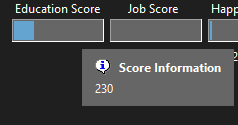
\includegraphics[width=0.4\textwidth]{images/implementation/scoresDisplay1.png}
    \caption{Scores progress bar with ToolTip visible}
    \label{fig:implementation-scoresDisplay1}
\end{figure}
This is the code which is run when the progress bars are updated.
\begin{lstlisting}[language=c, style=csharp, caption=Code to populate ToolTips showing score information]
ttMainToolTip.SetToolTip(prbEducationScore, prbEducationScore.Value.ToString());
ttMainToolTip.SetToolTip(prbHappinessScore, prbHappinessScore.Value.ToString());
ttMainToolTip.SetToolTip(prbJobScore, prbJobScore.Value.ToString());
ttMainToolTip.SetToolTip(prbLifeScore, prbLifeScore.Value.ToString());
ttMainToolTip.SetToolTip(prbMedicalScore, prbMedicalScore.Value.ToString());
\end{lstlisting}

\section{Disable clickables}
During testing, I realised that I have some clickable items (buttons etc) which are still enabled when the main character dies. To solve this, I am going to write a procedure which will disable all the clickable controls when it is run.\\
To do this, I will need a new procedure, shown below.
\begin{lstlisting}[language=c, style=csharp, caption=Disable clickables subroutine]
public void disableClickables()
{
    //procedure to disable all clickable elements on this form, for use when the main char dies.
    //There is no way to reverse this.

    btnAgeUp.Enabled = false;
    btnEduWithdraw.Enabled = false;
}
\end{lstlisting}
As the comments say, there is no way to overturn this procedure as this is only to be used at the very end of the game when the character is dead.\\
This worked the first time I tried this, shown below
\begin{figure}[H]
    \centering
    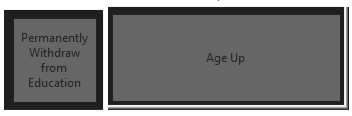
\includegraphics[width=0.4\textwidth]{images/implementation/disableClick1.jpg}
    \caption{Buttons disabled after the procedure above has been run}
    \label{fig:implementation-disableClick1}
\end{figure}
\noindent I am satisfied with this procedure as it works as expected.

\section{About Form}
This form is used to credit the assets I have downloaded from the internet. There are no programmatically elements to it apart from opening it. All design will be done in Visual Studio's designer.\\
Below is the form.
\begin{figure}[H]
    \centering
    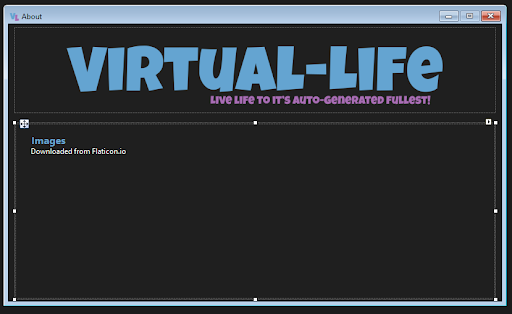
\includegraphics[width=0.8\textwidth]{images/implementation/aboutForm.png}
    \caption{About form design}
    \label{fig:implementation-aboutForm}
\end{figure}

\section{Crimes}
Now I need to add the code in which will let the player generate a random crime for their player to commit. It will be a very basic system, which gives the player no choice on what crime they commit and all the sentences will be between 1 and 12 years community service. For added humour, I won't be disabling this button until the character reaches a certain age as I feel it would be more amusing to have a 2 year old stealing a car.\\
See below for the code which runs the page on the tab control.
\begin{lstlisting}[language=c, style=csharp, caption=Procuedres which are run when the "Comit Random Crime" button is pressed]
private void btnCriCommitCrime_Click(object sender, EventArgs e)
{
    //first generate new crime then time of community service for it. 

    string[] crimes = { "Burgle a shop", "Steal a car", "Pirate a DVD" };
    int crimesLength = crimes.Length;
    int rand = randomNumber(0, crimesLength);
    int years = randomNumber(1, 12);
    string crimeText = "You committed a crime " + crimes[rand] + " and you recieved " + years.ToString() + " years community service.";
    generateEvent("Crime", crimes[rand], controlClass.InGameDate);
    updateCrimes();
}

public void updateCrimes()
{
    txtCriCrimeEvents.ResetText();
    for (int i = 0; i < controlClass.NextEvent; i++)
    {
        if (eventArray[i].Category == "Crimes")
        {
            txtCriCrimeEvents.Text = txtCriCrimeEvents.Text + Environment.NewLine + eventArray[i].DateHappened.ToShortDateString() + " - " + eventArray[i].Description;
        }

    }
}
\end{lstlisting}
This initially didn't work as expected as the crime only textbox doesn't show crimes however the main event box does. To rectify the issue with the crime only box, I corrected the line of code in \verb|updateCrimes()| in the if statement from “Crimes” to “Crime”. This works and produces the results I want.
\begin{figure}[H]
    \centering
    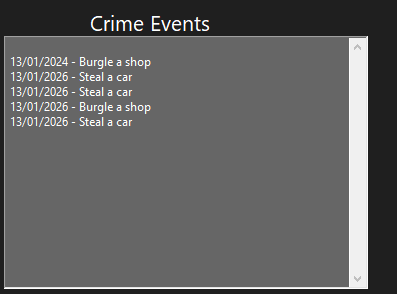
\includegraphics[width=0.4\textwidth]{images/implementation/crime1.png}
    \caption{Crime event box}
    \label{fig:implementation-crime1}
\end{figure}

\section{Customising Character}
To start working on this section, I need to design the form.
\begin{figure}[H]
    \centering
    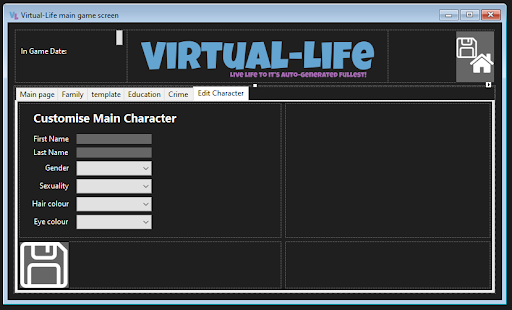
\includegraphics[width=0.8\textwidth]{images/implementation/customise1.png}
    \caption{Customise character options}
    \label{fig:implementation-customise1}
\end{figure}
\noindent This just has the customisation options at the moment and the save button. I still need to add the end life section to the right hand side of the screen. 
Now I need to add the code which will unlock these options once the main character has turned 13.
\begin{lstlisting}[language=c, style=csharp, caption=Yearly Check subroutine]
public void yearlyCheck()
{
    //this is a place which will run every time the mc ages up. If they are older than the specified age then will run code in relevant section.

    if(mainCharacter.Age >= 13)
    {
        //'unlock' character customisation screen.
        txtEditFirstName.Enabled = true;
        txtEditLastName.Enabled = true;
        cboEditGender.Enabled = true;
        cboEditSexuality.Enabled = true;
        cboEditEyeColour.Enabled = true;
        cboEditHairColour.Enabled = true;
    }
}
\end{lstlisting}
I have done this by writing a new procedure yearlyCheck() which gets run every time the player clicks age up. It will force the character customisation options to be enabled once the character turns 13. 
Next, I need to write the code which will populate these controls with the current information which the main character has.
\begin{lstlisting}[language=c, style=csharp, caption=Subroutine to update character customisaiton options]
public void updateCharCustomisationOptions()
{
    //fill all the Character Customisation option controls with current information from main char object
    txtEditFirstName.Text = mainCharacter.FirstName;
    txtEditLastName.Text = mainCharacter.LastName;
    cboEditGender.Text = mainCharacter.Gender;
    cboEditSexuality.Text = mainCharacter.Sexuality;
    cboEditHairColour.Text = mainCharacter.HairColour;
    cboEditEyeColour.Text = mainCharacter.EyeColour;
}
\end{lstlisting}
This procedure is called as part of the \verb|updateForms| procedure so it will be called every time age up is clicked.\\
Now I need to write the save button algorithm.
\begin{lstlisting}[language=c, style=csharp, caption=Save character customisation procedure]
public void saveCharCustomisationOptions()
{
    //if the contents of the text boxes etc is NOT null and is different to the current contents of the main character object, then it needs to be written into the object

    //start with the first name
    if(txtEditFirstName.Text != null && txtEditFirstName.Text != mainCharacter.FirstName)
    {
        mainCharacter.FirstName = txtEditFirstName.Text;
    }
    //next - do the last name
    if(txtEditLastName.Text != null && txtEditLastName.Text != mainCharacter.LastName)
    {
        mainCharacter.LastName = txtEditLastName.Text;
    }
    if(cboEditGender.Text != null && cboEditGender.Text != mainCharacter.Gender)
    {
        mainCharacter.Gender = cboEditGender.Text;
    }
    if(cboEditSexuality.Text != null && cboEditSexuality.Text != mainCharacter.Sexuality)
    {
        mainCharacter.Sexuality = cboEditSexuality.Text;
    }
    if(cboEditHairColour.Text != null && cboEditHairColour.Text != mainCharacter.HairColour)
    {
        mainCharacter.HairColour = cboEditHairColour.Text;
    }
    if(cboEditEyeColour.Text != null && cboEditEyeColour.Text != mainCharacter.EyeColour)
    {
        mainCharacter.EyeColour = cboEditEyeColour.Text;
    }
}
\end{lstlisting}
This half worked the first time I tried it. The edit aspect worked and the main display tab updated as I expected it to, however when I tried a null entry, the program allowed this to happen.
\begin{figure}[H]
    \centering
    
\includegraphics[width=0.4\textwidth]{images/implementation/customise2.png}
    \caption{Textbox on Customisation form}
    \label{fig:implementation-customise2}
\end{figure}

\begin{figure}[H]
    \centering
    
\includegraphics[width=0.4\textwidth]{images/implementation/customise3.png}
    \caption{Main info point on main game screen}
    \label{fig:implementation-customise3}
\end{figure}
\noindent To resolve this, I changed \verb|null| to \verb|""|. This worked and I now have a working character customisation page.\\
Next, I need to add the end life button. This will still generate a random reason for death.
First, I added the controls to the form then I added the code which will power it.\\
\begin{figure}[H]
    \centering
    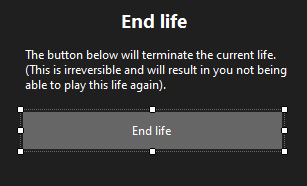
\includegraphics[width=0.4\textwidth]{images/implementation/endlife1.png}
    \caption{Button which ends the main characters life}
    \label{fig:implementation-endlife1}
\end{figure}
\begin{lstlisting}[language=c, style=csharp, caption=End life algorithm]
private void btnEndLife_Click(object sender, EventArgs e)
{
    DialogResult dialogResult = MessageBox.Show("Are you sure you want to end this life?", "End life", MessageBoxButtons.YesNo);
    if (dialogResult == DialogResult.Yes)
    {
        killMainCharacter();
    }
    else if (dialogResult == DialogResult.No)
    {
        //do something else
    }
}
\end{lstlisting}
As you can see from the code, it calls the same procedure that would be called if the main character was to die randomly.
\begin{figure}[H]
    \centering
    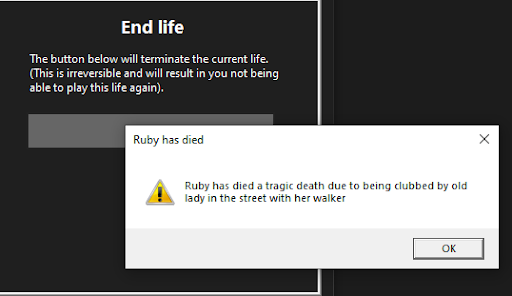
\includegraphics[width=0.6\textwidth]{images/implementation/endlife2.png}
    \caption{Output from pressing the end life button}
    \label{fig:implementation-endlife2}
\end{figure}
\noindent This worked as expected.

\section{Jobs}
The next part of the game which I am going to program is the jobs and employment feature.
To start off, I am going to follow my design and create a new tab page on the main tab control with the controls outlined in my design.
\begin{figure}[H]
    \centering
    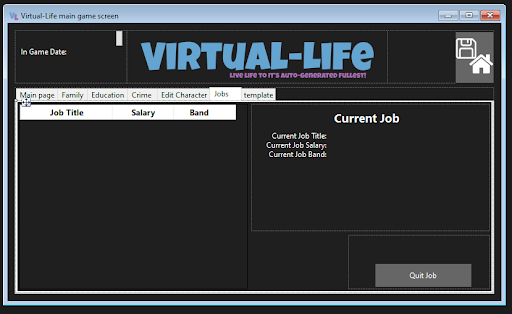
\includegraphics[width=0.8\textwidth]{images/implementation/jobs1.png}
    \caption{Design of the jobs form}
    \label{fig:implementation-jobs1}
\end{figure}
\noindent I then began to write the algorithm to generate jobs.
\begin{lstlisting}[language=c, style=csharp, caption=Algorithm to generate jobs]
 public Job generateJob (int band)
{
    string[] band1Job = { "Cleaner", "Wearhouse opperative", "Grocery picker", "Sahara delivery driver", "Burger flipper", "Hospital porter", "Community care worker", "Care assistant", "Handyperson", "Nursery assistant" };
    string[] band2Job = { "College security guard", "Pet groomer", "Engineer", "Secretary", "Line cook", "Plumber", "Cleaning company owner", "HR advisor", "Vehicle Technician", "Tanker driver" };
    string[] band3Jobs = { "Supervisor", "Senior Vehicle Technician", "Head of Resources", "Product manager", "Web developer", "Comms manager", "Software engineer", "Project manager", "Site manager", "Sales Director" };
    string[] band4Jobs = { "Store manager", "Finance Manager", "Site supervisor", "Nursing home manager", "IT Solutions Architect", "Senior API Developer", "Electrical Installation Lecturer", "Matron", "Defects manager", "Family Lawyer" };
    string[] band5Jobs = { "CEO", "Retail park manager", "Hotel manager", "Specialty doctor", "User interface designer", "SQL Developer", "DevOps engineer", "Senior Software consultant", "Executive head teacher", "Hospital director" };
    Job newJob = new Job();
    Random rnd = new Random();
    switch (band)
    {
        case 1:
            Salary = 17000;
            Band = 1;
            JobTitle = band1Job[rnd.Next(1, 9)];
            break;
        case 2:
            Salary = 34000;
            Band = 2;
            JobTitle = band2Job[rnd.Next(1, 9)];
            break;
        case 3:
            Salary = 51000;
            Band = 3;
            jobTitle = band3Jobs[rnd.Next(1, 9)];
            break;

        case 4:
            Salary = 68000;
            Band = 4;
            jobTitle = band4Jobs[rnd.Next(1, 9)];
            break;
        case 5:
            Salary = 150000;
            Band = 5;
            jobTitle = band5Jobs[rnd.Next(1, 9)];
            break;
    }
    return newJob;
}
\end{lstlisting}
I wrote some test code which would use a test button to generate a job and output the job title in a message box.
\begin{lstlisting}[language=c, style=csharp, caption=Procedure to call the generateJob function]
private void btnTestButton_Click(object sender, EventArgs e)
{
    Job newJob = new Job();
    newJob.generateJob(1);
    MessageBox.show(newJob.JobTitle);
}
\end{lstlisting}
When I ran the code, it gave me the following result; this means that my job generation code is working.
\begin{figure}[H]
    \centering
    \includegraphics[width=0.2\textwidth]{images/implementation/jobs2.png}
    \caption{Result from pressing test button}
    \label{fig:implementation-jobs2}
\end{figure}
\noindent Next, I need to write the algorithm which once the main character turns 18 generates band 1 jobs and populates the data grid view which they will be stored in. This is going to be done using a procedure - reshuffle Jobs. This is going to also be able to be called from the button which will reshuffle jobs. This button will initially be disabled, however once the main character turns 18, it will be enabled (in the same way as the edit character controls).
To start writing \verb|reshuffleJobs|, I will first generate the array of Job objects each containing different band jobs.It will then output these jobs to a \verb|DataGridView| control.
\begin{lstlisting}[language=c, style=csharp, caption=Reshuffle available jobs algorithm]
public void reshuffleJobs(int band)
{
    //first generate the jobs
    int maxNumb = 10;
    for (int i = 0; i < maxNumb; i++)
    {
        Job tempJob = new Job(); //make new instance of the object
        tempJob.generateJob(band); 
        availableJobs[i] = tempJob; //transfer the temp object into the array.
    }

    //now populate data grid view
    //first have to clear it
    dgvEmpAvailableJobs.Rows.Clear();
    dgvEmpAvailableJobs.Refresh();

    //use code from openldbws app to populate dgvEmpAvailableJobs

    //first, set var for which column contains which data
    int jtCol = 0;
    int salCol = 1;
    int bandCol = 2;

    //now loop through familyArray and populate dgvEmpAvailableJobs
    //as jobs are only ever generated and populated here - can use max number from job generation loop for loop here

    for (int x = 0; x < maxNumb; x++)
    {
        if (availableJobs[x].JobTitle != null)
        {
            int i = dgvEmpAvailableJobs.Rows.Add();
            dgvEmpAvailableJobs.Rows[i].Cells[jtCol].Value = availableJobs[x].JobTitle;
            dgvEmpAvailableJobs.Rows[i].Cells[salCol].Value = availableJobs[x].Salary;
            dgvEmpAvailableJobs.Rows[i].Cells[bandCol].Value = availableJobs[x].Band;
        }
    }
}
\end{lstlisting}
Which look like this
\begin{figure}[H]
    \centering
    \includegraphics[width=0.5\textwidth]{images/implementation/jobs3.png}
    \caption{Output of DataGridView control}
    \label{fig:implementation-jobs3}
\end{figure}
\noindent This worked first time as I copied and altered the code from the generation and population of the \verb|genericFamilyMember| object array and display for that.\\
Now I need to be able to “apply” for the job and display information about the job. First I added the apply button to the main form, then I wrote the code which will populate the label controls (displaying the current job information) and save the job which the main character has selected to the main character object.
\begin{lstlisting}[language=c, style=csharp, caption=Applying for job and updating job information procedures]
public void updateCurrentJobInformation()
{
    lblJobCurrentJobBand.Text = "Current Job Band: " + mainCharacter.JobBand.ToString();
    lblJobCurrentJobTitle.Text = "Current Job Title: " + mainCharacter.JobTitle.ToString();
    lblJobCurrentJobSalary.Text = "Current Job Salary: " + mainCharacter.JobSalary.ToString();

}

private void btnJobApplyForJob_Click(object sender, EventArgs e)
{
    mainCharacter.JobTitle = dgvEmpAvailableJobs.SelectedCells[0].Value.ToString();
    mainCharacter.JobSalary = Int32.Parse(dgvEmpAvailableJobs.SelectedCells[1].Value.ToString());
    mainCharacter.JobBand = Int32.Parse(dgvEmpAvailableJobs.SelectedCells[2].Value.ToString());
    updateCurrentJobInformation();
}
\end{lstlisting}
When I ran this for the first time, I got the following error: Object reference not set to an instance of an object with the displaying \verb|JobTitle| line highlighted.\\
To resolve this, I removed the \verb|.ToString()| method from the attributes which were already strings.
This worked, however I hadn't added the attribute titles to the code, which means it gets removed when the button is pressed. This gives me the result of
\begin{figure}[H]
    \centering
    \includegraphics[width=0.8\textwidth]{images/implementation/jobs4.png}
    \caption{Job page of main form (without label titles)}
    \label{fig:implementation-jobs4}
\end{figure}
\noindent Now I\textquotesingle ve added in the label titles, I get
\begin{figure}[H]
    \centering
    \includegraphics[width=0.4\textwidth]{images/implementation/jobs5.png}
    \caption{Correct display of job information}
    \label{fig:implementation-jobs5}
\end{figure}
\noindent I then tried to click on the apply for select job before I had loaded the available jobs, this resulted in the following error.
\begin{figure}[H]
    \centering
    \includegraphics[width=0.5\textwidth]{images/implementation/jobs6.png}
    \caption{Error from not selecting a job before applying for it}
    \label{fig:implementation-jobs6}
\end{figure}
\noindent To solve this, I added a \verb|Try-Catch| block with the exception handled by displaying a message to the user.
\begin{lstlisting}[language=c, style=csharp, caption=Apply for job procedure now with try-catch block]
 private void btnJobApplyForJob_Click(object sender, EventArgs e)
{
    try
    {
        mainCharacter.JobTitle = dgvEmpAvailableJobs.SelectedCells[0].Value.ToString();
        mainCharacter.JobSalary = Int32.Parse(dgvEmpAvailableJobs.SelectedCells[1].Value.ToString());
        mainCharacter.JobBand = Int32.Parse(dgvEmpAvailableJobs.SelectedCells[2].Value.ToString());
        mainCharacter.InJob = true;
        generateEvent("Job", "You applied for and got the job: " + mainCharacter.JobTitle, controlClass.InGameDate);
        updateCurrentJobInformation();
    } catch(Exception)
    {
        MessageBox.Show("Please select a job before applying for it.");
    }
}
\end{lstlisting}
This results in
\begin{figure}[H]
    \centering
    \includegraphics[width=0.8\textwidth]{images/implementation/jobs7.png}
    \caption{Result of applying for job without selecting a job after adding try-catch block}
    \label{fig:implementation-jobs7}
\end{figure}
\noindent Now I need to add the quit job code. As this button will be enabled even if the main character isn't currently in a job, I will use a try catch block again; to catch any exceptions.
\begin{lstlisting}[language=c, style=csharp, caption=Quit job algorithm]
private void button1_Click(object sender, EventArgs e) //quit job
{
    try
    {
        mainCharacter.JobTitle = "";
        mainCharacter.JobSalary = 0;
        mainCharacter.JobBand = 0;
        mainCharacter.InJob = false;
        mainCharacter.JobCurrentDuration = 0;
        generateEvent("Job", "You quit your job", controlClass.InGameDate);
    }
    catch (Exception)
    {
        MessageBox.Show("Please make sure you have a job before you try to quit it.");
    }
    updateCurrentJobInformation();
}
\end{lstlisting}
This worked as expected and gave me the results I wanted.
\begin{figure}[H]
    \centering
    \includegraphics[width=0.2\textwidth]{images/implementation/jobs8.png}
    \caption{Result of quitting a job in the events box}
    \label{fig:implementation-jobs8}
\end{figure}
\noindent Now that I have obtain and quit job code working, I need to write the job progression algorithms. This algorithm is going to work by looking at the \verb|JobCurrentTime| attribute of the main character and if the character has been in their current job for over a certain time then they will be offered the next band of job up. To start this algorithm, I will change the generate job procedure so if the main character has been in a job for less than 5 years the game will generate band 1 jobs.
This is the event handler code for when the button is pressed:
\begin{lstlisting}[language=c, style=csharp, caption=Start of the Reshuffle Job Board algorithm]
private void btnJobReshuffleJobBoard_Click(object sender, EventArgs e)
{
    if(mainCharacter.JobCurrentDuration < 5)
    {
        //can only get band 1 job
        reshuffleJobs(1);
    }
}
\end{lstlisting}
This worked so I can now add the second band code
\begin{lstlisting}[language=c, style=csharp, caption=Second iteration of the reshuffle job board algorithm]
private void btnJobReshuffleJobBoard_Click(object sender, EventArgs e)
{
    if(mainCharacter.JobCurrentDuration <= 5)
    {
        //can only get band 1 job
        reshuffleJobs(1);
    }
    else if (mainCharacter.JobCurrentDuration >=6 && mainCharacter.JobCurrentDuration <= 14)
    {
        //get band 2 job
        reshuffleJobs(2);
    }
}
\end{lstlisting}
This is also working and generating band 1 jobs while the main character has had a job for under 6 years then generating a band 2 job after that. As this is working, I can write the code to generate the rest of the bands of jobs.\\
This is working and producing the results I expect it to.\\
The next part of the jobs algorithm I need to program is the salary calculation This algorithm will be run every time the main character ages up, so the first thing which I need to do is check if the main character currently has a job. I am then able to write the code which will take the current salary, band and duration of which the main character has been in a job. \\
Below is the algorithm which will calculate the salary
\begin{lstlisting}[language=c, style=csharp, caption=Calculate job salary algorithm]
public void calculateSalary()
{
    Random rnd = new Random();
    //algorithm to generate the salary of the main character
    //needs to take into consideration the current band of job, base band of that salary and how long the mc has been in that job
    int salary = mainCharacter.JobSalary;
    int band = mainCharacter.JobBand;
    int duration = mainCharacter.JobCurrentDuration;

    if(mainCharacter.InJob == true)
    {
        //mc is in job so can now calc salary.
        int increaseAmount = rnd.Next(0, (band*duration));
        mainCharacter.JobSalary = salary + increaseAmount;
    }
}
\end{lstlisting}
To test this, I ran the program and found that the increases are too marginal for the game to be fun. I will need to increase the max increase amount by a factor of 10.
\begin{lstlisting}[language=c, style=csharp, caption=Salary increase amount calculation]
int increaseAmount = rnd.Next(0, (band*duration)*10);
\end{lstlisting}
This still isn't increasing the salary as much as I would like it to, so I am going to change the increase factor to 50. This is working much better and I am now happy with the salary calculation and salary increase algorithms.
Now I have built the jobs segment of the game, I need to remove the test settings, so players can only get jobs when they turn 18. I am going to do this in the same way that I did for the character customisation options, making the controls on the form default to be disabled, then every time age up is clicked they are enabled.
\begin{lstlisting}[language=c, style=csharp, caption=Age restriction for the jobs algorithms]
if (mainCharacter.Age >= 18)
{
    //'unlock' character job options
    btnJobApplyForJob.Enabled = true;
    btnJobQuitJob.Enabled = true;
    btnJobReshuffleJobBoard.Enabled = true;
}
\end{lstlisting}
This is working as I want it to.
Finally, the job score will simply be the duration which you have had the job for.
I have put the code for this in the \verb|updateCurrentJobInformation| procedure as this is both run every time a change is made to the employment situation and whenever the main character is aged up.
\begin{lstlisting}[language=c, style=csharp, caption=JobScore algorithm]
mainCharacterScores.JobScore = mainCharacter.JobCurrentDuration*4;
prbJobScore.Value = mainCharacterScores.JobScore;
\end{lstlisting}

\section{Medical}
This is going to be a very much behind the scenes algorithm which is going to randomly assign the medical score as well as enter some messages into the events box denoting what has happened medically. There will be no player interaction with this algorithm.
It will first get the main character\textquotesingle s current medical score, depending on what this is, the algorithm will generate a medical condition which will have a 5\% chance of affecting the main character. All the medical conditions generated will either be life-long or will never need to be referenced again, therefore I can save some processing by not needing to keep detailed information about each medical condition, meaning the game will be more lightweight to run.
Before I can write the algorithm, I'm going to have to change how the medical score is assigned when a new game is generated, it will have to be set to 100 not 0.
\begin{lstlisting}[language=c, style=csharp, caption=Medical score algorithms]
public void generateMedicalScore()
{
    Random rnd = new Random();
    int currentMedScore = mainCharacterScores.MedicalScore;
    if(currentMedScore == 100)
    {
        //has perfect health, 1/10 chance of it being lowered so can then be diseased.
        int chance = rnd.Next(0, 11);
        if(chance == 5)
        {
            currentMedScore = 99;
        }

    }
    if(currentMedScore < 100)
    {
        //can be diseased. 1 in 20 chance of getting disease
        int chance1 = rnd.Next(0, 21);
        if(chance1 == 12)
        {
            //is gonna be diseased
            string condition = getMedicalCondition();

            generateEvent("Medical","You " + condition, controlClass.InGameDate);

            mainCharacterScores.MedicalScore = mainCharacterScores.MedicalScore - rnd.Next(0, 50);

        }
    }
}

public string getMedicalCondition()
{
    string[] medicalConditions = {"broke your arm", "broke your leg", "stubbed your toe" };
    Random rnd = new Random();

    string returnString = medicalConditions[rnd.Next(0, medicalConditions.Length)];
    return returnString;
}
\end{lstlisting}
I tested this algorithm and it worked.
\begin{figure}[H]
    \centering
    \includegraphics[width=0.3\textwidth]{images/implementation/medical1.png}
    \caption{Result of medical condition generation}
    \label{fig:implementation-medical1}
\end{figure}
\noindent Now I just need to change the medical score value to 1000 and increase the decrease med score value.

\section{Partners}
The final main element of the game I need to program is the partner and courtship element. The courtship element will be an extremely simplified version of real life as every couple has a different path.
To start off with, I need to program the generation of a potential partner. There will be no lower age limit on this and the partner will have to be within 2 years of the main character. This will be generated in much the same way as the generic family members when a new game is created.
This is the code I have written in the main game screen form which is run whenever the button to generate potential partners is pressed.
\begin{lstlisting}[language=c, style=csharp, caption=Code to generate more potential partners]
private void btnParGenMore_Click(object sender, EventArgs e)
{
    generateAndPopulateMorePartners();
}

public void generateAndPopulateMorePartners()
{
    //Now create family members
    for (int i = 0; i < 10; i++)
    {
        DetailedCharacter tempFamily = new DetailedCharacter(); 
        tempFamily.generateDetailedChar(); 
        MessageBox.Show(tempFamily.FirstName);
    }
\end{lstlisting}
This calls the function in the detailed person class which looks like this.
\begin{lstlisting}[language=c, style=csharp, caption=Detailed char class code to generate a partner]
public DetailedCharacter generateDetailedChar()
{
    DetailedCharacter potential = new DetailedCharacter();
    FirstName = "Dave";
    return potential;
}
\end{lstlisting}
For testing, I have just programmed the first name to be “Dave”. This will allow me to make sure that everything is being called properly before I move onto the next part.\\
To test this so far, I can click the generate button and run the code.
\begin{figure}[H]
    \centering
    \includegraphics[width=0.2\textwidth]{images/implementation/partners1.png}
    \caption{Outcome from pressing generate button}
    \label{fig:implementation-partners1}
\end{figure}
\noindent This gave me the outcome which I expected. I will now move onto the display feature of the potential partners.
To do this, I will need to write the code which will add the generated temporary object to the array and write the code which will output the information to the user. The later I already have as I have been using \verb|DataGridViews| lots throughout the project, and the former I have in a different state which I can use here.\\
After running the code and once again confirming that the correct number of \verb|Dave|s appeared, the \verb|DataGridView| was populated as follows, confirming that the code is working this far.
\begin{figure}[H]
    \centering
    \includegraphics[width=0.4\textwidth]{images/implementation/partners2.png}
    \caption{Initial test of the data grid view used to show potential partners}
    \label{fig:implementation-partners2}
\end{figure}
Now I have the display working, I have a way to test the development of the different potential partners. The different combinations of sexuality and gender will be generated within the detailed character class.\\
Initially, I will be using a straight woman to start development.
\begin{lstlisting}[language=c, style=csharp, caption=Code to generate potential partners for a straight woman]
public DetailedCharacter generateDetailedChar(string gender, string sexuality, DateTime today)
{
    DetailedCharacter potential = new DetailedCharacter();

    if (gender == "Female")
    {
        if (sexuality == "Straight")
        {
            //generate a man
            FirstName = genMFN();
            LastName = genLN();
            Sexuality = "Straight";
            Gender = "Male";
            LivingStatus = true;
            DateOfBirth = today.AddDays(-rnd.Next(5840, 14600));
            Age = calcAge(DateOfBirth);
        }
    }
    FirstName = "Dave";
    return potential;
\end{lstlisting}
This worked as expected except for the fact I had left a line of debug code in from last time, hence all first names are “Dave”
\begin{figure}[H]
    \centering
    \includegraphics[width=0.4\textwidth]{images/implementation/partners3.png}
    \caption{Second test of displaying potential partners in the DataGridView}
    \label{fig:implementation-partners3}
\end{figure}
\begin{figure}[H]
    \centering
    \includegraphics[width=0.6\textwidth]{images/implementation/partners4.png}
    \caption{Final display of information about potneial partners in the DataGridView}
    \label{fig:implementation-partners4}
\end{figure}
\noindent This gives me the output which I am happy with.\\
The next thing I need to do is add the button which will initiate the relationship. To do this, I will need to add another column to the datagridview containing the index which the person is in the array, this means it will be really easy for me to access this and pull their information out of the \verb|DataGridView|.\\
Below is the code to ask the person on a date
\begin{lstlisting}[language=c, style=csharp, caption=Code to ask someone on a date]
private void btnAskOnDate_Click(object sender, EventArgs e)
{
    //basically the same as applying for a job
    try 
    {
        int index = Int32.Parse(dgvPartPotential.SelectedCells[4].Value.ToString());
        partner = potentialPartners[index];
        MessageBox.Show(partner.FirstName);
    }
    catch(Exception)
    {
        MessageBox.Show("Please select a partner before trying to go on a date with them.");
    }
    updatePartnerInformation();
}
\end{lstlisting}
This didn't work at first, as I was trying to cast one object to another without the proper conversion process, to get around this, I have had to change the class type from \verb|DetailedCharacter| to \verb|Partner| in all the code in this section so far.\\
This works and produces the result I was expecting, the first name of the person in a message box.
\begin{figure}[H]
    \centering
    \includegraphics[width=0.8\textwidth]{images/implementation/partners5.png}
    \caption{Output when clicking on ask partner on a date}
    \label{fig:implementation-partners5}
\end{figure}
\noindent Now I need to write the code which will generate the event for this
\begin{lstlisting}[language=c, style=csharp, caption=Code to create event saying that you have a new partner]
generateEvent("Relationships", "You asked " + partner.FirstName + " on a date and they said yes!", controlClass.InGameDate);
\end{lstlisting}
Now I need to write the code to save the partner's information to a file. This worked first time and produced the result I was expecting in the JSON file.\\
Now I will write the code for all the different combinations of gender and sexuality to produce different partners.
\begin{lstlisting}[language=c, style=csharp, caption=All the different combinations for generating different partners]
public Partner generateDetailedChar(string gender, string sexuality, DateTime today)
{
    Partner potential = new Partner();

    if (gender == "Female")
    {
        if (sexuality == "Straight")
        {
            //generate a man
            FirstName = genMFN();
            LastName = genLN();
            Sexuality = "Straight";
            Gender = "Male";
            LivingStatus = true;
            DateOfBirth = today.AddDays(-rnd.Next(5840, 14600));
            Age = calcAge(DateOfBirth);
        }else if (sexuality == "Homosexual")
        {
            //generate woman
            FirstName = genFFN();
            LastName = genLN();
            Sexuality = "Homosexual";
            Gender = "Female";
            LivingStatus = true;
            DateOfBirth = today.AddDays(-rnd.Next(5840, 14600));
            Age = calcAge(DateOfBirth);
        }
    }
    if (gender == "Male")
    {
        if (sexuality == "Homosexual")
        {
            //generate a man
            FirstName = genMFN();
            LastName = genLN();
            Sexuality = "Homosexual";
            Gender = "Male";
            LivingStatus = true;
            DateOfBirth = today.AddDays(-rnd.Next(5840, 14600));
            Age = calcAge(DateOfBirth);
        }
        else if (sexuality == "Straight")
        {
            //generate woman
            FirstName = genFFN();
            LastName = genLN();
            Sexuality = "Straight";
            Gender = "Female";
            LivingStatus = true;
            DateOfBirth = today.AddDays(-rnd.Next(5840, 14600));
            Age = calcAge(DateOfBirth);
        }
    }


    return potential;
}
\end{lstlisting}
This works as expected and generates me the combinations I was expecting it to. Now I can write the code which will display the partners information to the player.
\begin{lstlisting}[language=c, style=csharp, caption=Code to update the current partners information to the player]
public void updatePartnerInformation()
{
    if (mainCharacter.InRelationship == true)
    {
        lblPartFirstName.Text = "First Name: " + partner.FirstName;
        lblPartLastName.Text = "Last Name: " + partner.LastName;
        lblPartDateOfBirth.Text = "Date of Birth: " + partner.DateOfBirth.ToShortDateString();
        lblPartAge.Text = "Age: " + partner.Age.ToString();
    }
    else
    {
        lblPartFirstName.Text = "First Name: ";
        lblPartLastName.Text = "Last Name: ";
        lblPartDateOfBirth.Text = "Date of Birth: ";
        lblPartAge.Text = "Age: ";
    }
}
\end{lstlisting}
This worked the first time I tried it as I have written very similar code many times before.
Next, I will write the code which will allow the user to end the relationship with the partner.
\begin{lstlisting}[language=c, style=csharp, caption=Dump partner algorithm]
private void btnPartDump_Click(object sender, EventArgs e)
{
    mainCharacter.InRelationship = false;
    partner.FirstName = null;
    partner.LastName = null;
    partner.Sexuality = null;
    partner.Gender = null;
    partner.LivingStatus = false;
    partner.Age = 0;
    updatePartnerInformation();
}
\end{lstlisting}
This worked as I was expecting it to. The confirmation that the partner had been dumped is that the partner information area is cleared.\\
Finally, for the partner section, I will write the code which will increase the partners age by 1 year.
\begin{lstlisting}[language=c, style=csharp, caption=Increase age of partner]
if(mainCharacter.InRelationship == true)
{
    partner.Age = partner.Age + 1;
}
\end{lstlisting}
This also worked as I was expecting it to.
\chapter{Testing Post Development}
\label{chap:testPostDev}
Once I have finished programming my game, I will need to test all the elements of the app to ensure that I have (a) correctly programmed it, (b) there are no bugs, (c) the game meets my success criteria.

\section{Final Test Plan}

\begin{longtable}{p{0.05\textwidth}|p{0.15\textwidth}|p{0.2\textwidth}|p{0.2\textwidth}|p{0.2\textwidth}|p{0.05\textwidth}}
\textbf{Test $N\textsuperscript{\underline{o}}$} & \textbf{Test Title} & \textbf{Details} & \textbf{Expected Outcome} & \textbf{Final Outcome} & \textbf{Vid $N\textsuperscript{\underline{o}}$} \\
\hline
\endhead
1a & Loading the main menu & Start the application and wait for the first form to load. & The main menu is the first form to load. & The main menu is the first form to load. \tempText{Green}{Pass} & 1a \\
\hline
1b & Main menu buttons test 1 & From the main menu, press the 'New Game' button. & The main menu form closes and the new game creation tool form opens. & The main menu form closes and the new game creation tool form opens. \tempText{Green}{Pass} & 1b \\
\hline
1c & Main menu buttons test 2 & From the main menu, press the 'Show saved games' button. & The main menu form closes and the show saved games form opens. & The main menu form closes and the show saved games form opens. \tempText{Green}{Pass} & 1c \\
\hline
1d & Main menu buttons test 3 & From the main menu, press the 'Settings' button. & The main menu form closes and the settings form opens. & The button clicks but nothing happens as there is no settings form. \tempText{Red}{Fail} & 1d \\
\hline
1e & Main menu buttons test 4 & From the main menu, press the 'About' button. & The main menu form closes and the about form opens. & The main menu form closes and the about form opens. \tempText{Green}{Pass} & 1e \\
\hline
1f & Main menu accessibility test pt.1 & From the main menu form, maximise the window using the Windows Menu Bar. & All controls on the form will increase in size and increase the spacing between them. & All controls on the form will increase in size and increase the spacing between them. \tempText{Green}{Pass} & 1f \\
\hline
1g & Main menu accessibility test pt.2 & From the main menu form, restore down the window using the Windows Menu bar. & The controls on the form should respond by shrinking and keeping their spacing according to the new size of the window & The controls on the form should respond by shrinking and keeping their spacing according to the new size of the window \tempText{Green}{Pass} & 1g \\
\hline
2a & Generating new game with correct data & Create a new game, entering valid data and setting the save location. Then click the save button. & The app displays the main game screen form with the correct main character information displayed. & The app progresses to the main game screen. \tempText{Green}{Pass} & 2a \\
\hline
2b & Generating new game with some incorrect data & Create a new game, entering the wrong data types into the text boxes and setting the save location. For example, entering “123” into the first name field. & The app progresses as normal; numbers for names are valid entry. & The app progresses to the main game screen. \tempText{Green}{Pass} & 2b \\
\hline
2c & Generating new game leaving text boxes blank & Create a new game, without entering and information into any of the text boxes except save location. & The app will reject the input and instruct the player to enter the information or press the random button. & The app progresses to the main game screen. \tempText{Red}{Fail} & 2c \\
\hline
2d & Random generation & Create a new game and use the random button and setting the save location. & The app populates all the fields on the form with random data and then progresses onto the main game screen form. & The app populates all the fields on the form with random data and then progresses onto the main game screen form. \tempText{Green}{Pass} & 2d \\
\hline
2e & Re-roll random generation & Create a new game and use the random generation button, then press it again and setting the save location. & The app will generate two different sets of random information and display them sequentially. They should be different. The app will then progress onto the main game screen. & The app will generate two different sets of random information and display them sequentially. They should be different. The app then progresses onto the main game screen. \tempText{Green}{Pass} & 2e \\
\hline
2f & New game form accessibility & Move between the controls without using mouse. & Click in the first textbox then navigate through the form by using keyboard only. & Had to click in first textbox to enter the tab chain. Was able to move between character information successfully, however unable to move into save location or select the save button so had to use mouse. \tempText{Red}{Fail} & 2f \\
\hline
2g & New game form accessibility pt.2 & From the main menu form, maximise the window using the Windows Menu Bar. & All the controls on the form should respond by growing and keeping their spacing according to the size of the window. & Some of the controls resized, however the majority didn't. \tempText{Red}{Fail} & 2g \\
\hline
2h & New game form accessibility pt.3 & From the main menu form, restore down the window using the Windows Menu bar. & The controls on the form should respond by shrinking and keeping their spacing according to the new size of the window & All controls responded by shrinking and sorting their spacing according to the new size of the window. \tempText{Green}{Pass} & 2h \\
\hline
2i & Not specifying a save location & Generate a random game and click save without specifying a save location & The game rejects the input and displays a message box instructing users to select a save location. & The game rejects the input and displays a message box instructing users to select a save location. \tempText{Green}{Pass} & 2i \\
\hline
3a & Loading from file with correct file placement & Load the game from the a folder with all the files intact and correctly placed. & The app will load the data then display the main game screen. & The app behaves as expected and opens the correct data. \tempText{Green}{Pass} & 3a \\
\hline
3b & Loading from file with missing files & Load the game from a folder with missing files. & The app will say that files are missing and not load the game. It will clear the form ready for the next attempt. & The app crashes and displays a runtime error. \tempText{Red}{Fail} & 3b \\
\hline
3c & Loading from file with a completely wrong folder & Load the game from a random folder that doesn’t contain any of the correct files. & The app will say that files are missing and not load the game. It will clear the form ready for the next attempt. & The app crashes and displays a runtime error. \tempText{Red}{Fail} & 3c \\
\hline
3d & Show saved games form accessibility test pt.1 & From the main menu form, maximise the window using the Windows Menu Bar. & All the controls on the form should respond by growing and keeping their spacing according to the size of the window. & Some of the controls resized, however the majority didn't. \tempText{Red}{Fail} & 3d \\
\hline
3e & Show saved games form accessibility test pt.2 & From the main menu form, restore down the window using the Windows Menu bar. & The controls on the form should respond by shrinking and keeping their spacing according to the new size of the window. & All controls responded by shrinking and sorting their spacing according to the new size of the window. \tempText{Green}{Pass} & 3e \\
\hline
4a & Pressing the save and home button & From the main game screen, press the save and home button. & The app will save the data to the files then close the main game screen form and open the main menu form. & The app saved the data to the files then close the main game screen form and open the main menu form. \tempText{Green}{Pass} & 4a \\
\hline
4b & Pressing the 'age up' button & Click the age up button. & The age up algorithm is followed correctly; with no unnecessary alerts to the player. The scores should also be re-calculated and their displays updated. & The age up algorithm is followed correctly. No unnecessary alerts are displayed to the user. The score displays change. \tempText{Green}{Pass} & 4b \\
\hline
4c & Changing tabs & Using the tab menu bar control, click from tab to tab. & When clicking from tab-to-tab, the correct controls only should be displayed. & When clicking from tab-to-tab, the correct controls only should be displayed. \tempText{Green}{Pass} & 4c \\
\hline
4d & Main game screen accessibility test pt.1 & From the main game screen form, maximise the window using the Windows Menu Bar. & All the controls on the form should respond by growing and keeping their spacing according to the size of the window & The controls on the form do nothing. \tempText{Red}{Fail} & 4d \\
\hline
4e & Main game screen accessibility test pt.2 & From the main game screen form, restore down the window using the Windows Menu bar. & The controls on the form should respond by shrinking and keeping their spacing according to the new size of the window & All controls responded by shrinking and sorting their spacing according to the new size of the window. \tempText{Green}{Pass} & 4e \\
\hline
5a & Family tab - alive select & From the family tab, select an alive family member. & The family member information populates accordingly with 'N/A' for reason and date of death. & The family member information populates accordingly with 'N/A' for reason and date of death. \tempText{Green}{Pass} & 5a \\
\hline
5b & Family tab - select dead & From the family tab, select a dead family member. & The family member information populates accordingly with correct reason and date of death & The family member information populates accordingly with correct reason and date of death. \tempText{Green}{Pass} & 5b \\
\hline
6a & Choice box & Play though the game which will trigger the choice box to appear in time with education events. & The choice box appears at the correct times throughout the game with the correct information on it. & The choice box appears at the correct times throughout the game with the correct information on it. \tempText{Green}{Pass} & 6a \\
\hline
6b & Education events are visible in the correct places & After entering the age bracket where education events are generated, the education events should appear both in the main event box and in the education specific box & The education events will appear in the main event box and in the education specific event box & The education events appear in the main event box and in the education specific event box. \tempText{Green}{Pass} & 6b \\
\hline
6c & Education information is correct on the form & Before pressing age up, observe the education information and observe again after pressing age up & The education information (points, current situation) are correct on the form & The education information (points, current situation) are correct on the form. \tempText{Green}{Pass} & 6c \\
\hline
6d & Permanently withdraw from education button prevents any more education events from being generated & Press the 'Permanently Withdraw From Education' button & No more education events will generate & No more education related events get generated. \tempText{Green}{Pass} & 6d \\
\hline
7a & Commit random crime button & Press the 'Commit random crime' button & A random crime will be generated and displayed & A random crime is generated and displayed. \tempText{Green}{Pass} & 7a \\
\hline
7b & Crime event box showing the correct data only & After pressing commit random crime button, observe the crime event box & Only crime events are displayed in the crime event box. & Only crime events are displayed in the crime event box. \tempText{Green}{Pass} & 7b \\
\hline
8a & Edit character unlocks correctly & Before the main character is 13, the edit character options should be 'locked' and after they turn 13, they should be 'unlocked' & After main character turns 13, the edit character options unlock & After main character turns 13, the edit character options unlock. \tempText{Green}{Pass} & 8a \\
\hline
8b & Edit character saves data when correct data is entered & Enter correct data into the edit character options, then press save. & The main game tab should update accordingly & The main game tab updates accordingly. \tempText{Green}{Pass} & 8b \\
\hline
8c & Edit character rejects erroneous data & Empty one of the textbox controls on the edit character options, then press save & The game rejects the input. & The game rejects the input. \tempText{Green}{Pass} & 8c \\
\hline
8d & end life works as expected press yes & Press the end life button then press 'yes' on the dialogue box & The game should trigger the end life algorithm and 'kill' the main character & The game triggers the end life algorithms and 'kills' the main character. \tempText{Green}{Pass} & 8d \\
\hline
8e & end life works as expected. press no & Press the end life button then press 'no' on the dialogue box & The game should return to the edit character screen. & The game returns to the edit character screen. \tempText{Green}{Pass} & 8e \\
\hline
9a & Refresh available jobs once & Press the 'Refresh available jobs' button & The game should generate a new set of jobs. & The game generates a new set of jobs. \tempText{Green}{Pass} & 9a \\
\hline
9b & Refresh available jobs twice & Press the 'Refresh available jobs' button twice & The game should generate two different sets of jobs. & The game generates two different sets of jobs. \tempText{Green}{Pass} & 9b \\
\hline
9c & Select an available job and apply & Highlight an available job and press the 'apply' button & The game should set the current job information to the job which has just been applied for and should generate a suitable event. & The game sets the current job information to the job which has just been applied for and generates a suitable event. \tempText{Green}{Pass} & 9c \\
\hline
9d & Quit job & Press the quit job button & The game should clear the current job information. & The game clears the current job information. \tempText{Green}{Pass} & 9d \\
\hline
9e & Apply for a new job while main character currently has one & Select and apply for a job while the main character currently has one & The game should reject this and display a message box to the player saying they need to quit their current job first. & The game allows the main character to apply for a job without quitting their current one first. \tempText{Red}{Fail} & 9e \\
\hline
10a & Generate one set of potential partners & From the partners screen, press 'Generate more partners' button & The game should generate a new set of potential partners & The game generates a new set of potential partners. \tempText{Green}{Pass} & 10a \\
\hline
10b & Generate two sets of potential partners & From the partners screen, press 'Generate more partners' button twice & The game should generate two different sets of potential partners. & The game generates two different sets of potential partners. \tempText{Green}{Pass} & 10b \\
\hline
10c & Select a potential partner and take on date & From the partners screen, select a potential partner and take press take on date & The game should populate the current partner information and generate an event. & The game populates the current partner information and generates an event. \tempText{Green}{Pass} & 10c \\
\hline
10d & Dump the partner & When you have a partner, press the 'dump' button & The game should clear the current partner information. & The game clears the current partner information. \tempText{Green}{Pass} & 10d \\
\hline
11a & Generating partners after changing main characters gender and/or sexuality & After changing the main characters gender and/or sexuality, press the generate more partners button & The game should  generate the correct potential partners for the main characters new gender and/or sexuality & The game generates the correct potential partners for the main characters new gender and/or sexuality. \tempText{Green}{Pass} & 11a \\
\hline
12a & Death & Play through the game and wait for death to occur. & The game should randomly kill all people in the game. Family members should have an event generated and the main character should have a message box displayed to the player & The game randomly kills people in the game and displays it appropriately. \tempText{Green}{Pass} & FL1; FL2 \\
\hline
\end{longtable}
\textit{NB: The saved game data from video FL2 is available in the Appendix \ref{chap:exampleSaveD}}

\begin{multicols}{2}
[
\section{User Acceptance Testing}
For the final testing for my project, I will ask some of my friends \& classmates who fit into the stakeholders category to test my project and give me feedback. Their findings are listed below and will be discussed in the Evaluation chapter.
\subsection{Findings from User Acceptance Testing}
]
\textbf{Liked:}
\begin{itemize}
    \item reasons for death
    \item the changes in lengths of life
    \item the random generation of names
    \item the random generation of crimes
    \item the random generation of jobs
    \item the silly death reasons
    \item \verb|TAB| key working to move between controls on character creation form
\end{itemize}

\textbf{Didn't like:}
\begin{itemize}
    \item that the same death could occur twice in the same game
    \item the death frequency
    \item the age gap possibilities between the partner and main character
    \item when main character died at age 1
    \item even if both the parents have died, the school events reference them
\end{itemize}
\textbf{Suggested Improvements:}
\begin{itemize}
    \item buttons need labels as well as icons
    \item make the label controls on the choice box clickable too
    \item neaten the 'Save \& Home' icon so they don't overlap
    \item the main character should automatically get a job when the turn 18
\end{itemize}
\end{multicols}

\begin{multicols}{2}
[
\subsection{Observations from User Acceptance Testing}
These are observations I made while watching other people play my game:
]
\begin{itemize}
    \item Quit band 1 jobs quite frequently
    \item Didn't attempt to edit the character
    \item Didn't say but inferred liked progress bars for score display
    \item Flicked between tabs lots
    \item Users struggled with using the app without any guidance or input from me
    \item Users stayed on the main page mostly, not interacting with other elements of the game
\end{itemize}
\end{multicols}
\subsection{Evidence of my testers testing}
Shown below are screenshots of direct messages with my testers, evidencing that they were involved in the user acceptance testing.

\begin{figure}[H]
    \begin{minipage}{0.45\textwidth}
        \begin{figure}[H]
        \centering
        \includegraphics[width=0.9\textwidth]{images/evalutation/Evidence from Poppy.jpg}
        \caption{Evidence of tester 1 - Poppy}
        \label{fig:evidencePoppy}
        \end{figure}
    \end{minipage} \hfill
    \begin{minipage}{0.45\textwidth}
        \begin{figure}[H]
        \centering
        \includegraphics[width=0.9\textwidth]{images/evalutation/Evidence from Nuala.jpg}
        \caption{Evidence of tester 1 - Nuala}
        \label{fig:evidenceNuala}
        \end{figure}
    \end{minipage}
\end{figure}

\chapter{Evaluation}
Once I had fully constructed my circuit, I am able to connect it to the power supply and evaluate what I have produced against my success criteria.
\section{Evaluating against Specification}
\begin{itemize}
    \item \textbf{The voltmeter will measure in volts and range from 0V to 5V, in 0.1V increments.}\\ When the voltmeter works, this is achieved. However as the voltmeter doesn't work reliably this point \tempText{red}{cannot be marked as achieved}.
    \item \textbf{The voltmeter will have a sample rate of 1KHz $\pm 400Hz$ times per second. This will be produced by Schmitt Astable with a frequency of 1KHz.}\\ From testing the clock subsystem, I know that the frequency of the clock is $1.36KHz$. This is a suitable deviation from the original success criteria (as it is an increase of less than 400Hz), meaning the clock pulses 1360 times per second. Therefore this point \tempText{Green}{can be marked as achieved}.
    \item \textbf{The voltmeter is accurate to within $\pm0.1V$.}\\ From testing the final circuit, I have found out that when it works, it is accurate within my specified bounds but when it doesn't work it is extremely inaccurate. Therefore this point \tempText{orange}{can be marked as partially achieved}.
    \item \textbf{The voltmeter takes less than 0.5 seconds to adjust its output once a change in voltage is detected.}\\ Despite the fact that the voltmeter was unreliable, I was able to measure the frequency of the clock. This frequency would mean that the clock could complete a full ramp in less than 0.5 seconds. Therefore this point \tempText{Green}{marked as achieved}.
    \item \textbf{The voltmeter should take a +5v, 0V and -5V (within ±0.5V) input.}\\ These are the inputs required for the DAC subsystem, therefore this point \tempText{Green}{can be marked as achieved}.
    \item \textbf{The voltmeter will be easy to use.}\\ From testing and asking the opinions of those who have tested my voltmeter for me, I have found that the voltmeter is easy to use. Therefore this point \tempText{Green}{can be marked as achieved}.
    \item \textbf{The voltage will output to two 7-segment displays; one for the units and one for the tenths.} \\ As seen in my full layout image, there are two 7-segment displays, one of which is used for units and the other for tenths. Therefore this point \tempText{Green}{can be marked as achieved}.
    \item \textbf{The entire circuit will only require human input to connect the analogue voltage.}\\ When the circuit is working, this point is achieved. However as the circuit doesn't work all of the time, this point \tempText{orange}{can be marked as partially complete}.
    \item \textbf{The voltmeter should be as efficient as possible, reducing heat dissipated to the environment.}\\ As my circuit is using a low voltage and current input, there isn't much energy to be dissipated. This low energy input requirement is partially due to the fact that I chose to use CMOS chips rather than TTL. TTL require a much higher operating voltage and current therefore they dissipate a much higher amount of energy. Therefore this point \tempText{Green}{can be marked as achieved}.
\end{itemize}
From evaluating against my specification, I can conclude that this project was not a complete success as only 66\% of the specification points were met. \newline For my project to have been a success, I would have needed an 75\% achievement rate of my success criteria. This would have meant 7 of the points would have to be achieved.

\section{Improvements}
To improve this project, I would troubleshoot further into the cause of the latches not clocking at the right time, then work to fix that issue. Assuming that this is the only issue I come into, then that would allow me to mark the remaining 4 success criteria points as achieved.\newline
A further improvement I could make is to take my layout on breadboards, and use a digital tool to convert it into a PCB. This would reduce the overall physical layout of the circuit as well as reduce the chance for a component to be knocked out. Furthermore, this would improve the noise performance of the circuit and allow for a better grounding arrangement. This would also allow me to implement a better timing system as it would be simpler to construct.

\section{Conclusion}
In conclusion, my system did not meet all of the specification points I put together before constructing it. This means it is not a functioning voltmeter. This was an extremely challenging project however once I understood how the subsystems worked, I was able to design and build them using the knowledge I gained from the theory modules of the course. The most challenging aspect was troubleshooting the many issues I ran into, especially the noise on the output from the DAC.

\appendix
\chapter{Full Code Listing}
\label{chap:fullCodeListing}

\section{Forms}

\subsection{Main Menu}
\subsubsection{[FILE]Form1.cs}
\lstinputlisting[style=csharp, language=c, caption=FILE/Form1.cs]{Components/code/forms/Form1.cs}
\subsubsection{[FILE]Form1.Designer.cs}
\lstinputlisting[style=csharp, language=c, caption=FILE/Form1.Designer.cs]{Components/code/forms/Form1.Designer.cs}

\subsection{About}
\subsubsection{[FILE]frmAbout.cs}
\lstinputlisting[style=csharp, language=c, caption=FILE/frmAbout.cs]{Components/code/forms/frmAbout.cs}
\subsubsection{[FILE]frmAbout.Designer.cs}
\lstinputlisting[style=csharp, language=c, caption=FILE/frmAbout.Designer.cs]{Components/code/forms/frmAbout.Designer.cs}

\subsection{Choice Box}
\subsubsection{[FILE]frmChoiceBox.cs}
\lstinputlisting[style=csharp, language=c, caption=FILE/frmChoiceBox.cs]{Components/code/forms/frmChoiceBox.cs}
\subsubsection{[FILE]frmChoiceBox.Designer.cs}
\lstinputlisting[style=csharp, language=c, caption=FILE/frmChoiceBox.Designer.cs]{Components/code/forms/frmChoiceBox.Designer.cs}

\subsection{Loading Bar}
\subsubsection{[FILE]frmLoadingBar.cs}
\lstinputlisting[style=csharp, language=c, caption=FILE/frmLoadingBar.cs]{Components/code/forms/frmLoadingBar.cs}
\subsubsection{[FILE]frmLoadingBar.Designer.cs}
\lstinputlisting[style=csharp, language=c, caption=FILE/frmLoadingBar.Designer.cs]{Components/code/forms/frmLoadingBar.Designer.cs}

\subsection{Main Game Screen}
\subsubsection{[FILE]frmMainGameScreen.cs}
\lstinputlisting[style=csharp, language=c, caption=FILE/frmMainGameScreen.cs]{Components/code/forms/frmMainGameScreen.cs}
\subsubsection{[FILE]frmMainGameScreen.Designer.cs}
\lstinputlisting[style=csharp, language=c, caption=FILE/frmMainGameScreen.Designer.cs]{Components/code/forms/frmMainGameScreen.Designer.cs}

\subsection{Show Saved Games}
\subsubsection{[FILE]frmShowSavedGames.cs}
\lstinputlisting[style=csharp, language=c, caption=FILE/frmShowSavedGames.cs]{Components/code/forms/frmShowSavedGames.cs}
\subsubsection{[FILE]frmShowSavedGames.Designer.cs}
\lstinputlisting[style=csharp, language=c, caption=FILE/frmShowSavedGames.Designer.cs]{Components/code/forms/frmShowSavedGames.Designer.cs}

\section{Classes}

\subsection{Control Class}
\subsubsection{[FILE]ControlClass.cs}
\lstinputlisting[style=csharp, language=c, caption=FILE/controlClass.cs]{Components/code/class/ControlClass.cs}

\subsection{Detailed Character}
\subsubsection{[FILE]DetailedCharacter.cs}
\lstinputlisting[style=csharp, language=c, caption=FILE/DetailedCharacter.cs]{Components/code/class/DetailedCharacter.cs}

\subsection{Event}
\subsubsection{[FILE]Event.cs}
\lstinputlisting[style=csharp, language=c, caption=FILE/Event.cs]{Components/code/class/Event.cs}

\subsection{Generic Family Member}
\subsubsection{[FILE]GenericFamilyMember.cs}
\lstinputlisting[style=csharp, language=c, caption=FILE/GenericFamilyMember.cs]{Components/code/class/GenericFamilyMember.cs}

\subsection{Job}
\subsubsection{[FILE]Job.cs}
\lstinputlisting[style=csharp, language=c, caption=FILE/Job.cs]{Components/code/class/Job.cs}

\subsection{Main Character}
\subsubsection{[FILE]MainCharacter.cs}
\lstinputlisting[style=csharp, language=c, caption=FILE/MainCharacter.cs]{Components/code/class/MainCharacter.cs}

\subsection{Partner}
\subsubsection{[FILE]Partner.cs}
\lstinputlisting[style=csharp, language=c, caption=FILE/Partner.cs]{Components/code/class/Partner.cs}

\subsection{Person}
\subsubsection{[FILE]Person.cs}
\lstinputlisting[style=csharp, language=c, caption=FILE/Person.cs]{Components/code/class/Person.cs}

\subsection{Score}
\subsubsection{[FILE]Score.cs}
\lstinputlisting[style=csharp, language=c, caption=FILE/Score.cs]{Components/code/class/Score.cs}


\section{Supporting Files}

\subsection{Program}
\subsubsection{[FILE]Program.cs}
\lstinputlisting[style=csharp, language=c, caption=FILE/Program.cs]{Components/code/Program.cs}

\chapter{Example Game Saved Data}
\label{chap:exampleSaveD}
This is the saved game data produced from the game in video FL2.\\
\textit{NB: These files have been passed through a \href{https://jsonformatter.curiousconcept.com/}{JSON File Formatter} to improve the readability of the data. The game saves the data as a single line without any formatting etc.}
\section{Files}

\subsection{Control Class}
\subsubsection{[FILE]controlClass.json}
\lstinputlisting[style=pseudo, caption=FILE/controlclass.json]{Components/exampleGameData/controlClass.json}

\subsection{Event Array}
The file below has been altered further from the formatted file (described above) and original file which the game produces. The game generates 1000 elements to the \verb|eventArray|, all of these, no matter if they are null get written out to the file, resulting in a file with 5002 lines (which takes up about 95 pages in this document). From a space efficiency point of view, the file has been trimmed, only showing 1 null event. There are 957 more in the original file.
\subsubsection{[FILE]eventArray.json}
\lstinputlisting[style=pseudo, caption=FILE/eventArray.json]{Components/exampleGameData/eventArrayTrimmed.json}

\subsection{Family Array}
In a similar way to the \verb|eventArray| file, the \verb|familyArray| file has also been altered by removing 26 null elements from the array.
\subsubsection{[FILE]familyArray.json}
\lstinputlisting[style=pseudo, caption=FILE/familyArray.json]{Components/exampleGameData/familyArrayTrimmed.json}

\subsection{Main Character}
\subsubsection{[FILE]mainCharacter.json}
\lstinputlisting[style=pseudo, caption=FILE/mainCharacter.json]{Components/exampleGameData/mainCharacter.json}

\subsection{Main Character Scores}
\subsubsection{[FILE]mainCharacterScores.json}
\lstinputlisting[style=pseudo, caption=FILE/mainCharacterScores.json]{Components/exampleGameData/mainCharacterScores.json}

\subsection{Partner}
\subsubsection{[FILE]partner.json}
\lstinputlisting[style=pseudo, caption=FILE/partner.json]{Components/exampleGameData/partner.json}
\chapter{References}

\section{Resources Used For Implementation}
Listed below are resources which were used to aid programming during the implementation phase of the project.
\begin{itemize}
    \item \href{https://docs.microsoft.com/en-us/dotnet/csharp/}{Microsoft C\# documentation}
    \item \href{https://stackoverflow.com/}{Stack Overflow}
    \item \href{https://www.codeproject.com/}{Code Project}
    \item \href{https://www.geeksforgeeks.org/}{Geeks For Geeks}
    \item \href{http://net-informations.com/}{Net Informations}
    \item \href{https://www.codegrepper.com/}{Code Grepper}
    \item \href{https://www.w3schools.com/}{W3 Schools}
    \item \href{https://www.dotnetperls.com/}{Dot Net Perls}
    \item \href{https://www.c-sharpcorner.com/}{C Sharp Corner}
\end{itemize}

\section{Newtonsoft Package}
I used the \verb|Newtonsoft.JSON| package during implementation to aid me with handling JSON files. Listed below are the resources I used to aid me with this.
\begin{itemize}
    \item \href{https://www.newtonsoft.com/json}{Newtonsoft JSON home page}
    \item \href{https://www.newtonsoft.com/json/help/html/SerializingJSON.htm}{Serializing JSON documentation}
    \item \href{https://www.newtonsoft.com/json/help/html/DeserializeAnonymousType.htm}{Deserialize Anonymous Type documentation}
\end{itemize}

\chapter{Screenshots Of Forms}
\label{app:ScreenshotsOfForms}

\section{Main Menu}
\begin{figure}[H]
    \centering
    \includegraphics[width=0.9\textwidth]{images/forms/menu.png}
    \caption{Annotated main menu form}
    \label{fig:forms-menu}
\end{figure}

\section{New Game}
\begin{figure}[H]
    \centering
    \includegraphics[width=0.9\textwidth]{images/forms/newGame.png}
    \caption{Annotated new game form}
    \label{fig:forms-newGame}
\end{figure}

\section{Show Saved Games}
\begin{figure}[H]
    \centering
    \includegraphics[width=0.9\textwidth]{images/forms/showSavedGames.png}
    \caption{Annotated show saved games form}
    \label{fig:forms-showSavedGames}
\end{figure}

\section{About}
\begin{figure}[H]
    \centering
    \includegraphics[width=0.9\textwidth]{images/forms/about.png}
    \caption{Annotated about form}
    \label{fig:forms-about}
\end{figure}

\section{Choice Box}
\begin{figure}[H]
    \centering
    \includegraphics[width=0.9\textwidth]{images/forms/choice-box.png}
    \caption{Annotated choice box form}
    \label{fig:forms-choiceBox}
\end{figure}

\section{Main Game Screen}
\subsection{Main Page}
\begin{figure}[H]
    \centering
    \includegraphics[width=0.9\textwidth]{images/forms/main-main.png}
    \caption{Annotated main game tab of main game screen form}
    \label{fig:forms-main-main}
\end{figure}

\subsection{Crime}
\begin{figure}[H]
    \centering
    \includegraphics[width=0.9\textwidth]{images/forms/main-crime.png}
    \caption{Annotated crime tab of main game screen form}
    \label{fig:forms-main-crime}
\end{figure}

\subsection{Edit Character}
\begin{figure}[H]
    \centering
    \includegraphics[width=0.9\textwidth]{images/forms/main-edit.png}
    \caption{Annotated edit character tab of main game screen form}
    \label{fig:forms-main-edit}
\end{figure}

\subsection{Education}
\begin{figure}[H]
    \centering
    \includegraphics[width=0.9\textwidth]{images/forms/main-education.png}
    \caption{Annotated education tab of main game screen form}
    \label{fig:forms-main-education}
\end{figure}

\subsection{Family}
\begin{figure}[H]
    \centering
    \includegraphics[width=0.9\textwidth]{images/forms/main-family.png}
    \caption{Annotated family tab of main game screen form}
    \label{fig:forms-main-family}
\end{figure}

\subsection{Jobs}
\begin{figure}[H]
    \centering
    \includegraphics[width=0.9\textwidth]{images/forms/main-jobs.png}
    \caption{Annotated jobs tab of main game screen form}
    \label{fig:forms-main-jobs}
\end{figure}

\subsection{Partners}
\begin{figure}[H]
    \centering
    \includegraphics[width=0.9\textwidth]{images/forms/main-partners.png}
    \caption{Annotated partners tab of main game screen form}
    \label{fig:forms-main-partners}
\end{figure}

\chapter{Full Index}
\begingroup
\let\clearpage\relax
\tableofcontents
\endgroup

\listoffigures
\lstlistoflistings

\end{document}
